\documentclass{article}

\usepackage{pdfpages}

\usepackage[hidelinks]{hyperref}

\usepackage{array}
\usepackage{tabularx}

\usepackage{comment}

\usepackage{tcolorbox}

\usepackage{graphicx}
\usepackage{subcaption}

\usepackage{amsmath}

\usepackage{float}

\usepackage[export]{adjustbox}

\usepackage[margin=1.25in]{geometry}

\newtcbox{\inlinecode}{on line, boxrule=0pt, boxsep=0pt, top=2pt, left=2pt, bottom=2pt, right=2pt, colback=gray!15, colframe=white, fontupper={\ttfamily \footnotesize}}

\begin{document}
\pagenumbering{gobble}

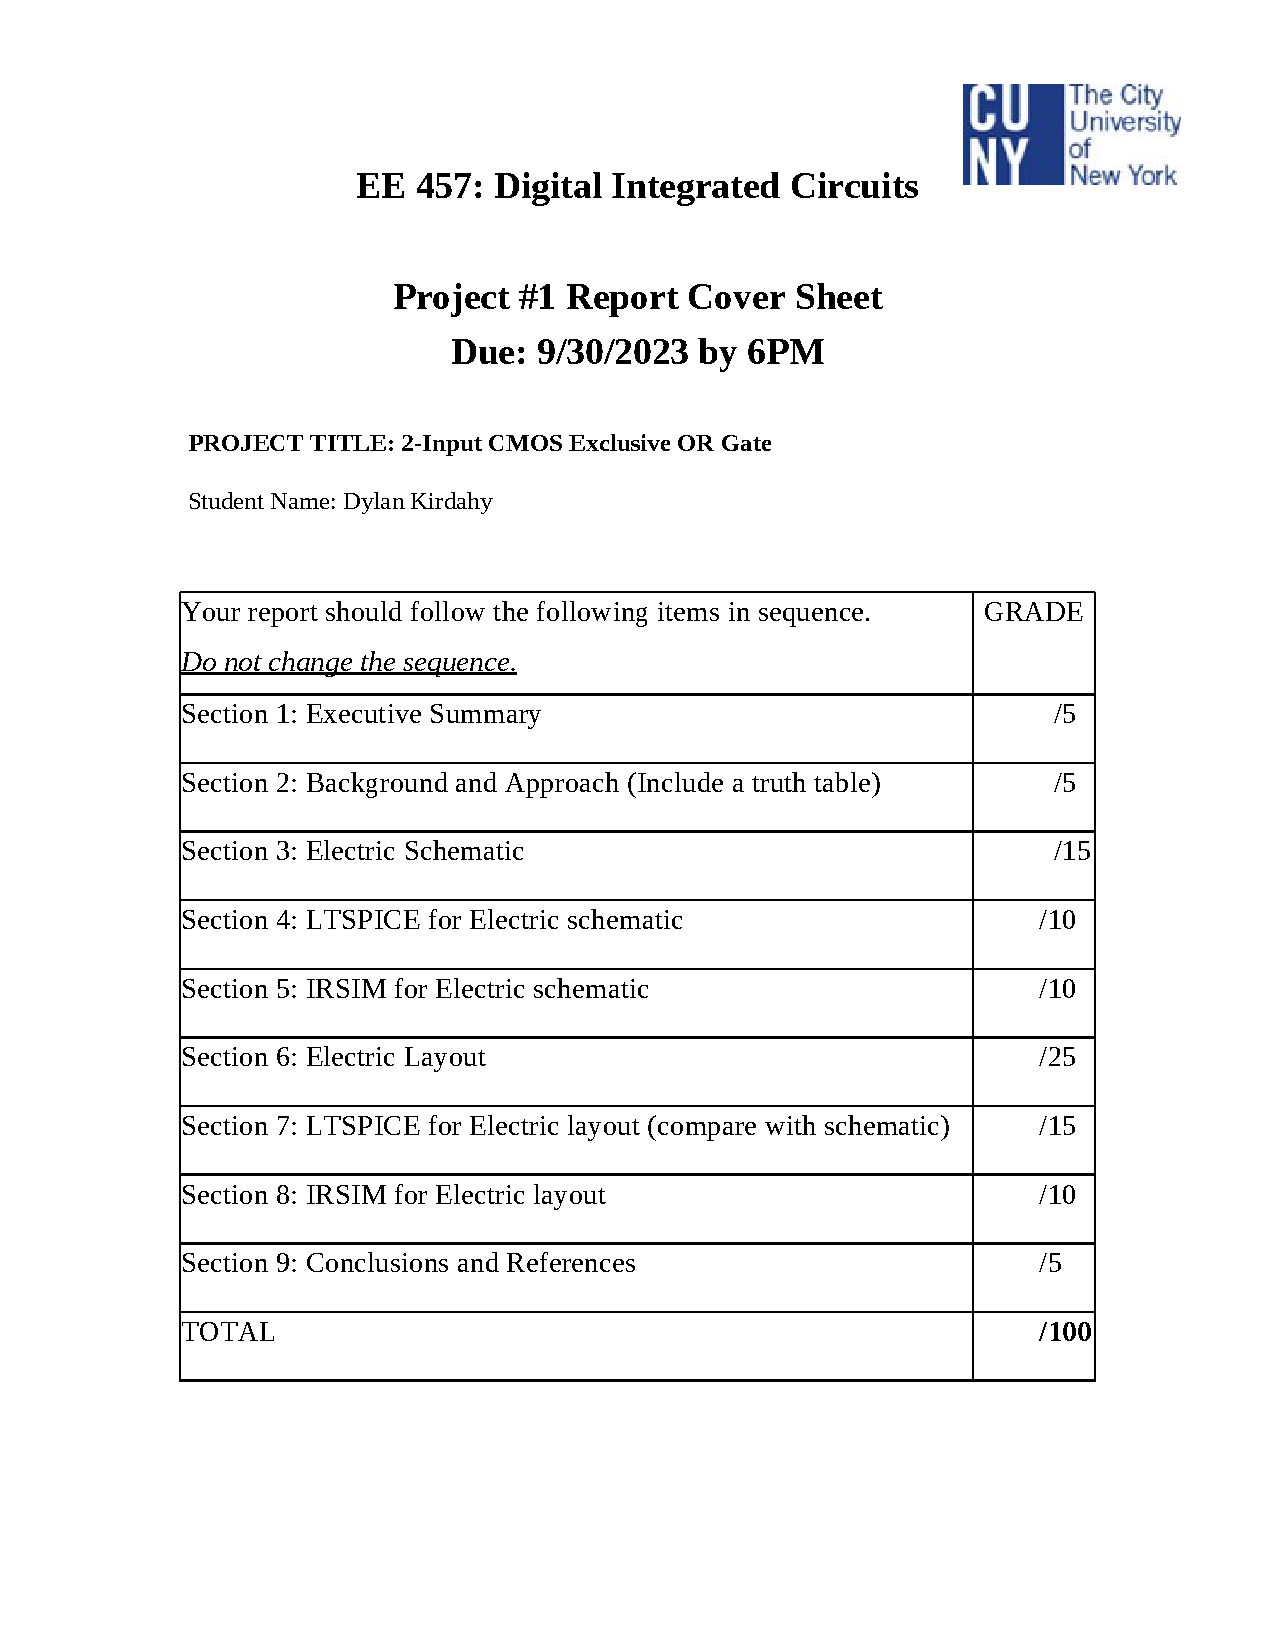
\includepdf[pages=-,scale=1,pagecommand={}]{project-1-cover-sheet.pdf}

\tableofcontents

\newpage
\pagenumbering{arabic}

\section{Executive Summary}
  \paragraph{}
  The goal of this project is to design an XOR gate CMOS integrated circuit using the design software Electric. The process of designing the chip involves starting with the boolean logic that makes up an XOR gate, turning that logic into a functioning schematic using CMOS logic, and then turning that schematic into a finished layout. Then, both the schematic and the layout are simulated in both LTSpice and IRSIM to confirm that they function properly, and finally measurements can be taken in LTSpice to further validate the design. Ultimately, this project is an introduction to the process of turning requirements into a finished design and then validating the design using the tools we have learned from creating the inverter.

\section{Background}
  \paragraph{}
  Designing an IC that performs the function of an XOR gate begins with an understanding of what an XOR gate does. The operation, denoted as $F=A \oplus B$ is a boolean logic function that takes inputs A and B and outputs a 0 if they are the same and 1 if they are dissimilar. This behavior can be seen in Table \ref{table:xor}. The symbol for the XOR gate is shown in Figure \ref{fig:symbol}. We can break down this logic into the following boolean expressions: $F=A \oplus B = A\overline{B}+\overline{A}B=(A+B)(\overline{A}+\overline{B})$


  \begin{table}[H]
    \centering
    \footnotesize
    \begin{tabular}{|c|c|c|}
      \hline
      \textbf{Input A} & \textbf{Input B} & \textbf{Output F} \\
      \hline
      0 & 0 & 0 \\
      \hline
      0 & 1 & 1 \\
      \hline
      1 & 0 & 1 \\
      \hline
      1 & 1 & 0 \\
      \hline
    \end{tabular}
    \caption{Truth Table for the XOR gate.}
    \label{table:xor}
  \end{table}


  \begin{figure}[H]
    \centering
    
\includegraphics[width=0.3\linewidth, frame]{images/xor-symbol.png}
    \caption{The symbol for the XOR gate.}
    \label{fig:symbol}
  \end{figure}

\section{Approach}
  \paragraph{}
  I chose to start designing the CMOS logic using the function $F=A\overline{B}+\overline{A}B$. The first thing to do is to invert the function, since the output of a CMOS circuit is inverted. Therefore we must invert F and then implement that function in the pull down network. Using De Morgan's Law, we get: $\overline{F}=\overline{A\overline{B}+\overline{A}B}=\overline{A\overline{B}}\cdot\overline{\overline{A}B}=(\overline{A}+B)(A+\overline{B})$ Therefore $(\overline{A}+B)(A+\overline{B})$ will be implemented on the NMOS side. We do this by putting the transistors in parallel for OR and in series for AND. For the pull up network, we put the PMOS transistors in series for OR and in parallel for AND. I sketched out the resulting circuit, as shown in Figure \ref{fig:sketch1}.

  \begin{figure}[H]
    \centering
    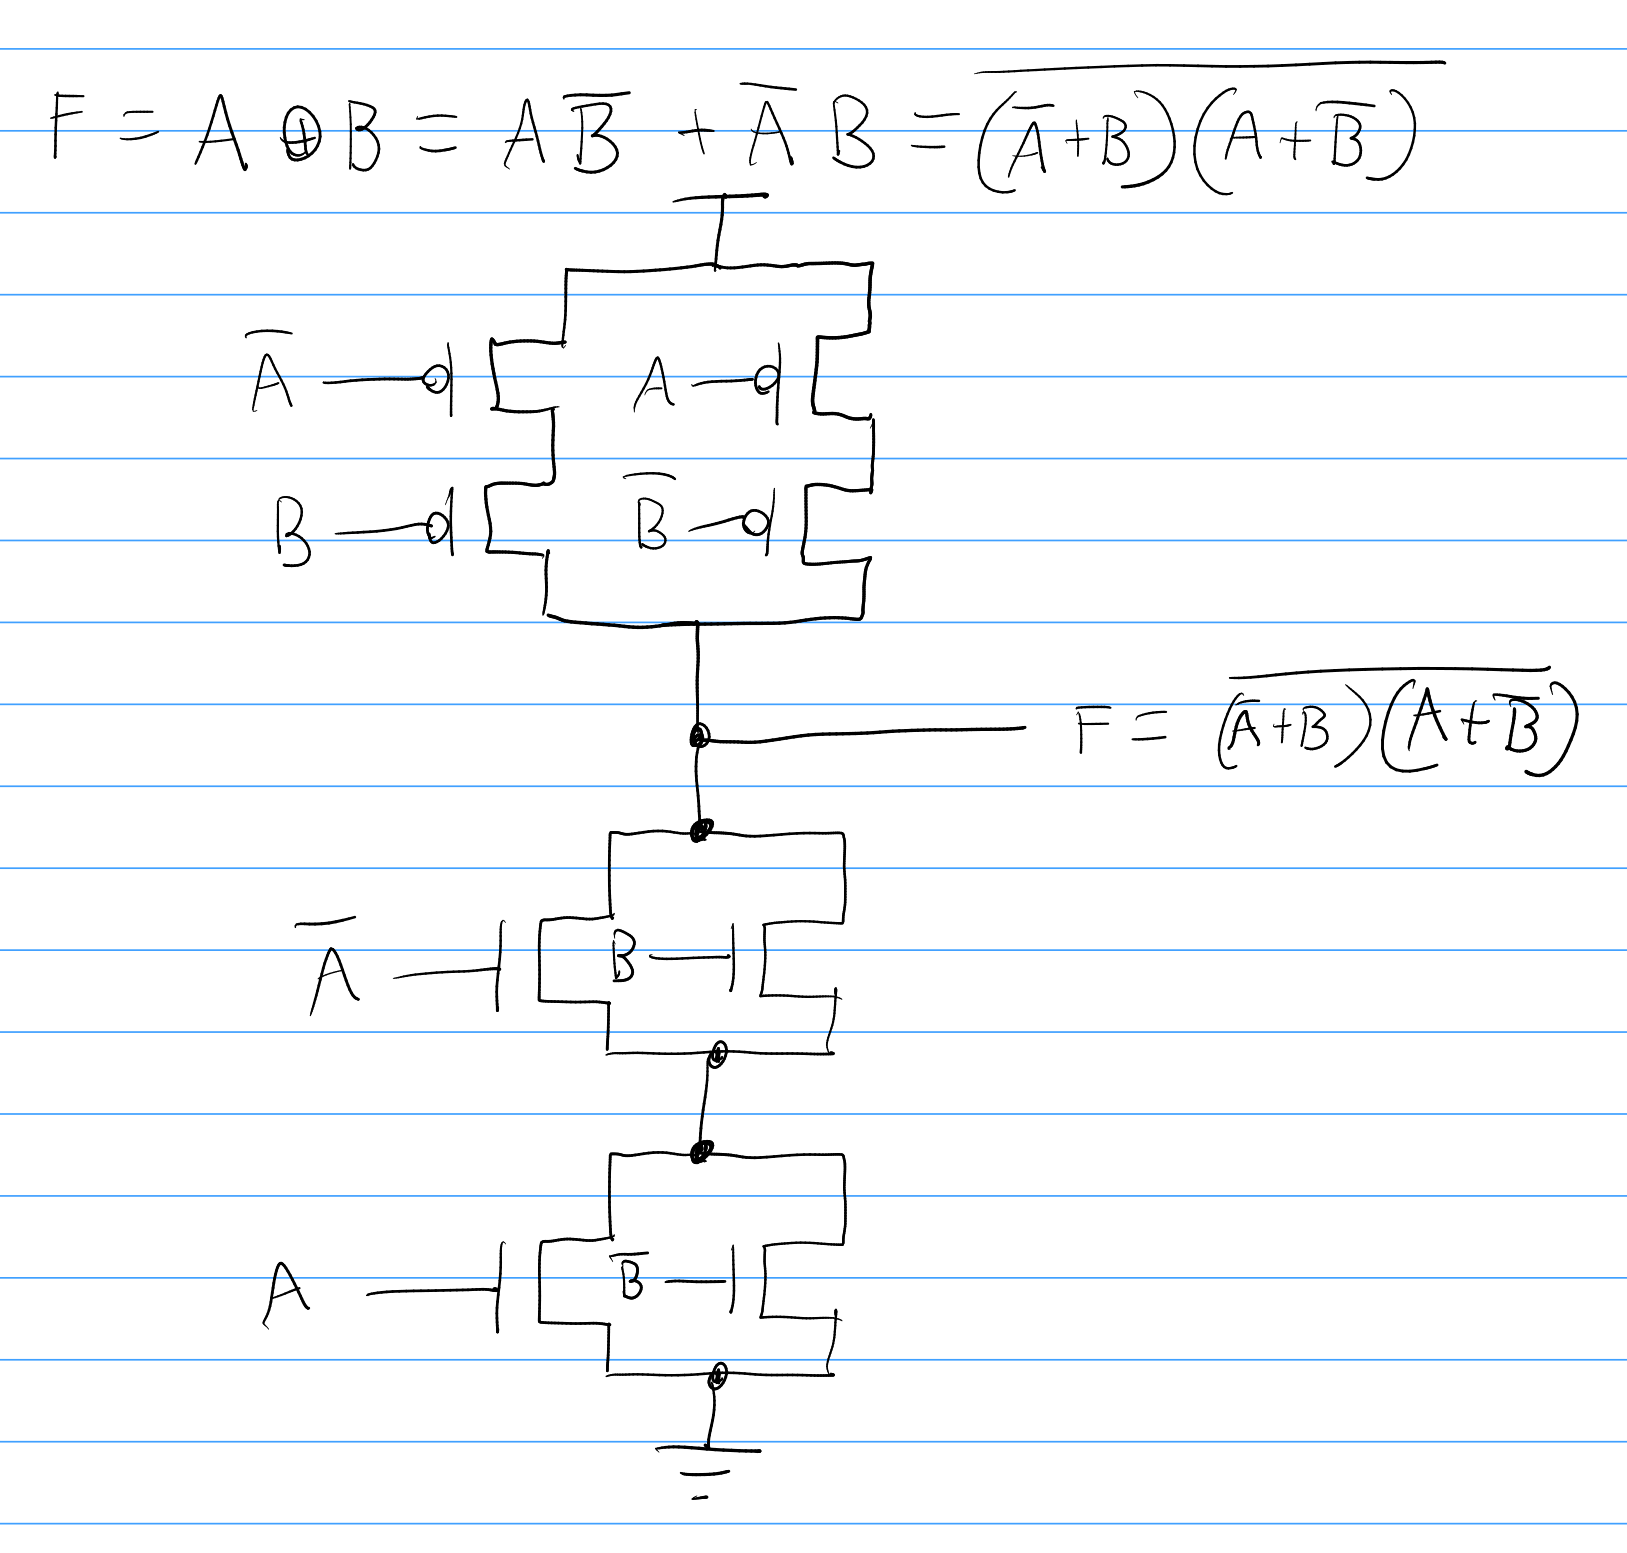
\includegraphics[width=0.7\linewidth, frame]{screenshots/schematic-sketch-1.png}
    \caption{A sketch of the PUN and PDN for implementing the XOR gate.}
    \label{fig:sketch1}
  \end{figure}

  \paragraph{}
  Since we are only given $A$ and $B$ as inputs and not $\overline{A}$ and $\overline{B}$ as well, we have to invert A and B for the inputs where $\overline{A}$ and $\overline{B}$ are necessary. This requires two inverters at the inputs, as shown in the sketch in Figure \ref{fig:sketch2}.


  \begin{figure}[H]
    \centering
    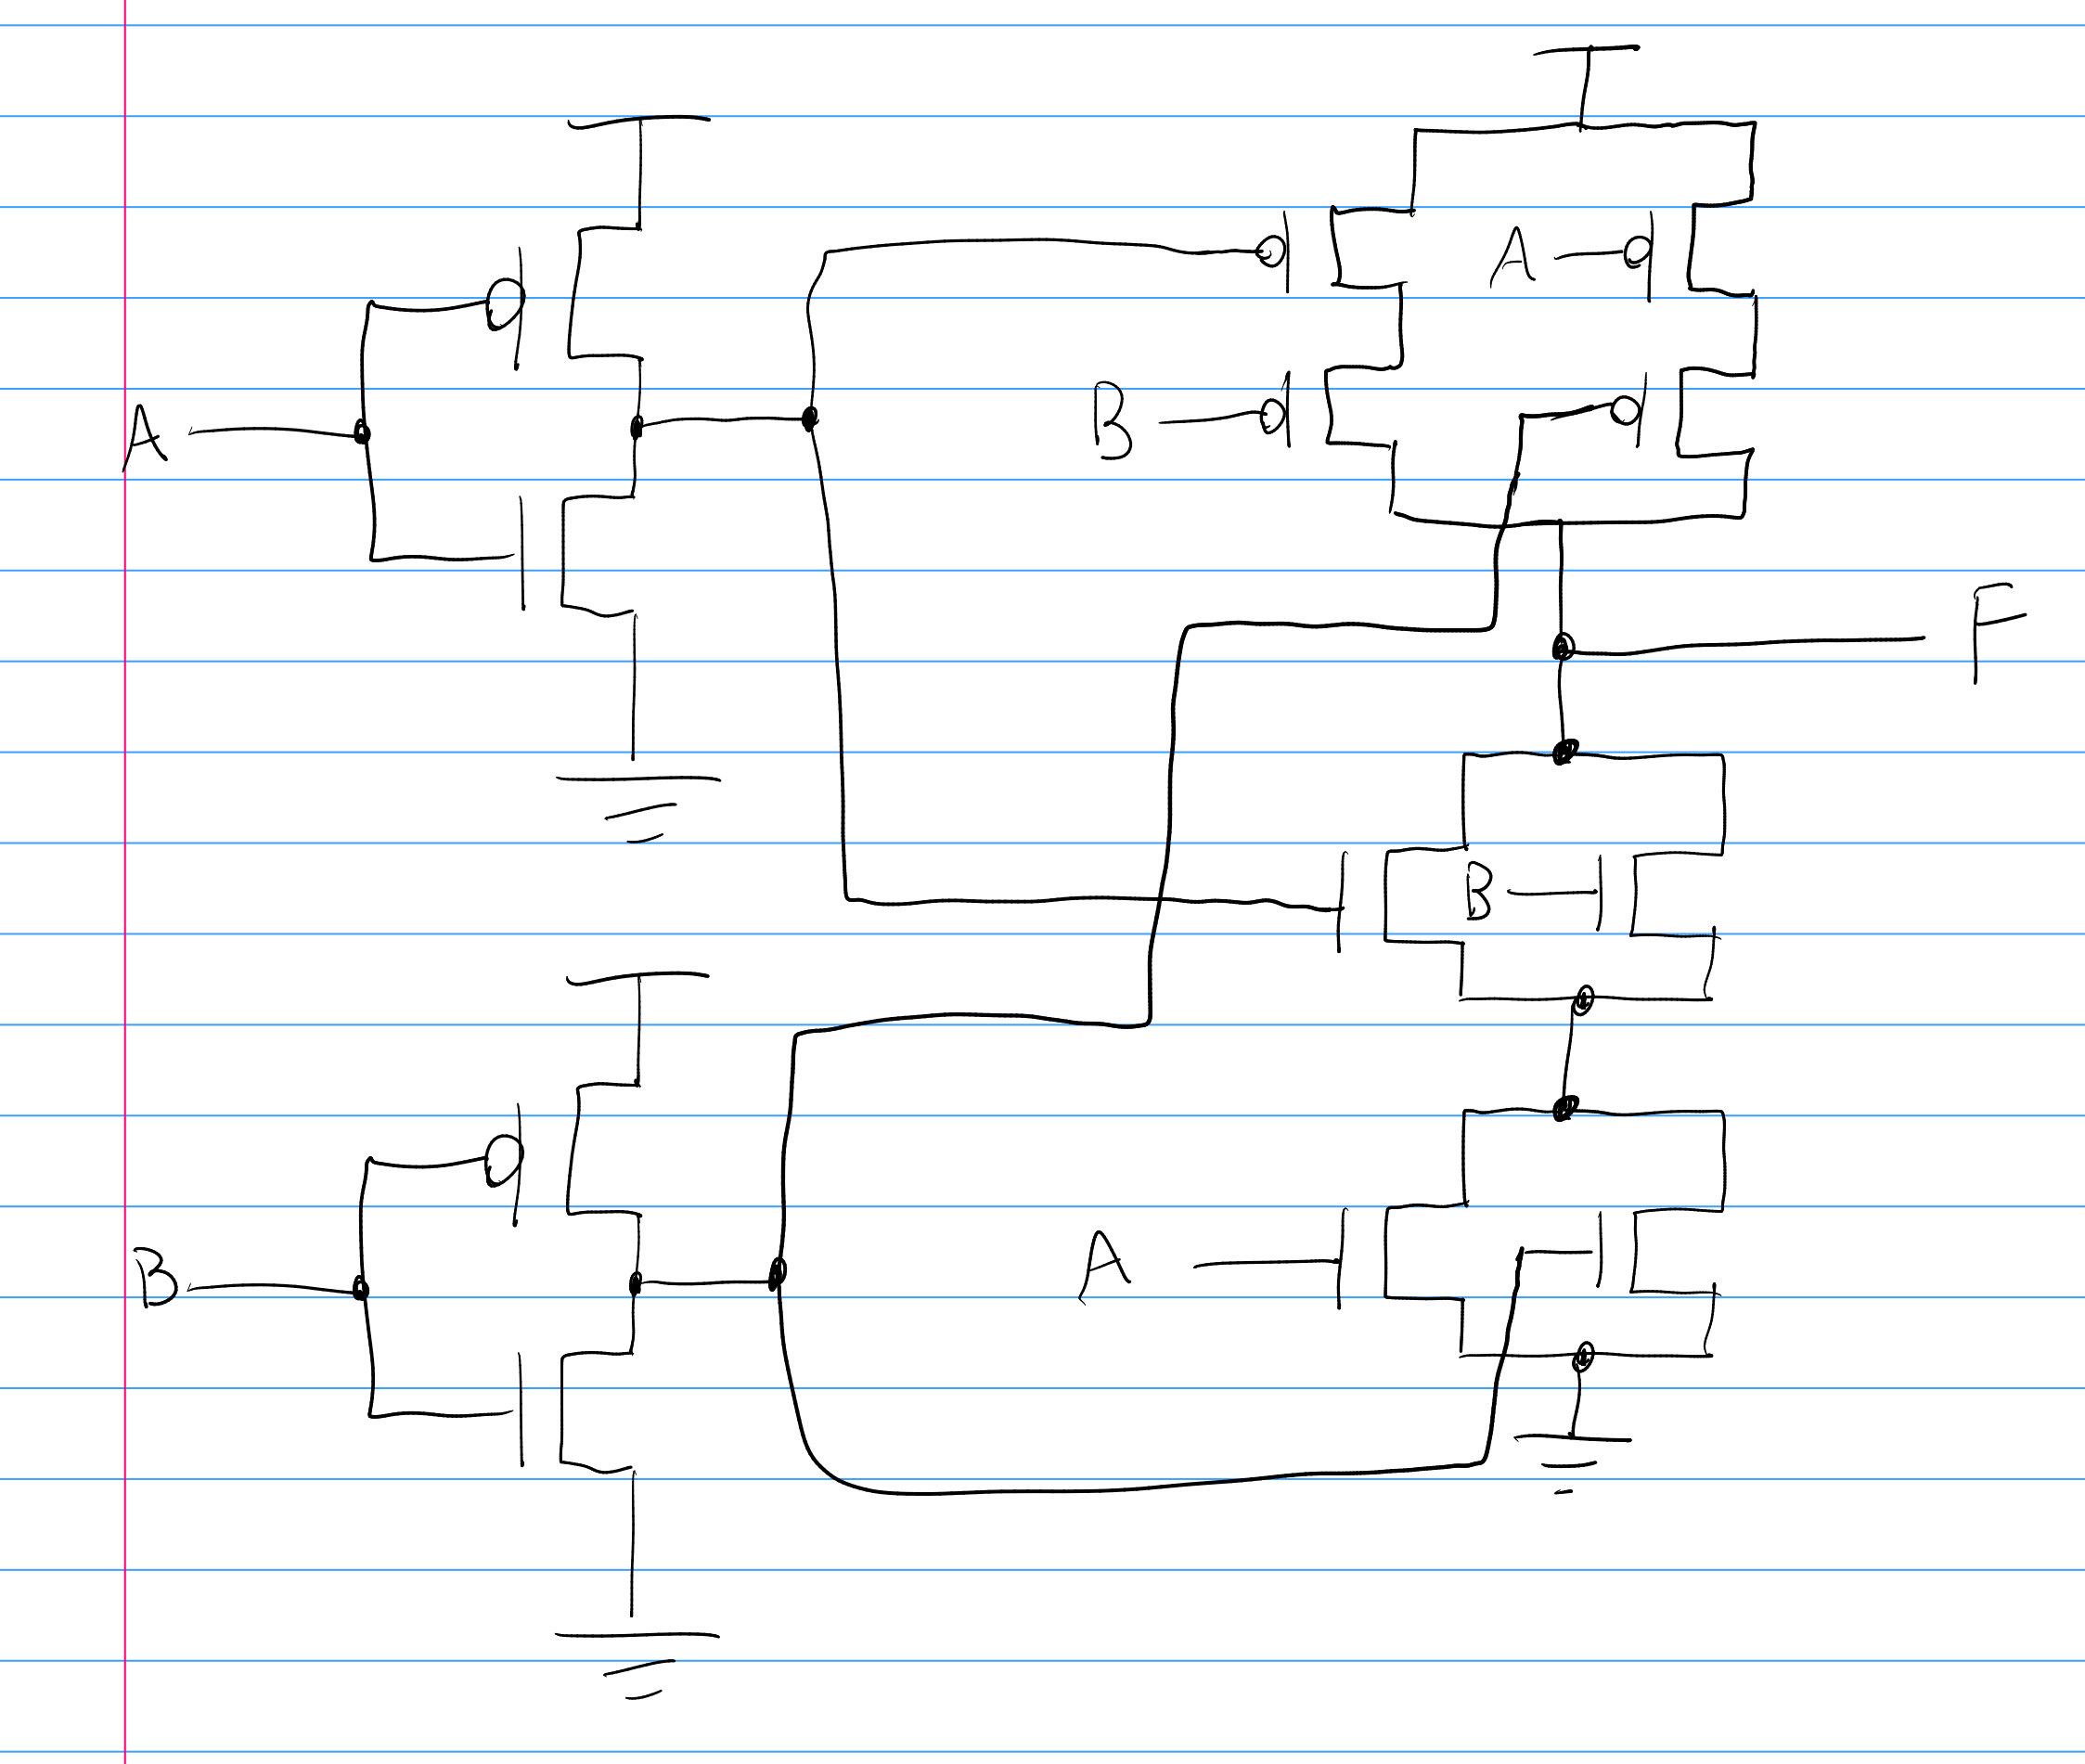
\includegraphics[width=0.7\linewidth, frame]{screenshots/schematic-sketch-2.png}
    \caption{A sketch of the XOR gate in CMOS logic.}
    \label{fig:sketch2}
  \end{figure}

\section{Schematic in Electric}

  \paragraph{}
  The sketch of the circuit was then built in the schematic design portion of Electric. The final schematic can be seen in Figure \ref{fig:schem}. The various nets that feed into the PUN and PDN are labeled to make the schematic easier to read. The transistors were initially chosen to be 8$\lambda$ wide and 2$\lambda$ long for PMOS and 4$\lambda$ wide and 2$\lambda$ because those are the dimensions that worked best for the inverter that we designed previously. However, we were told to make the PMOS transistors and NMOS transistors the same size, so I made them all 8$\lambda$ wide and 2$\lambda$.

  \begin{figure}[H]
    \centering
    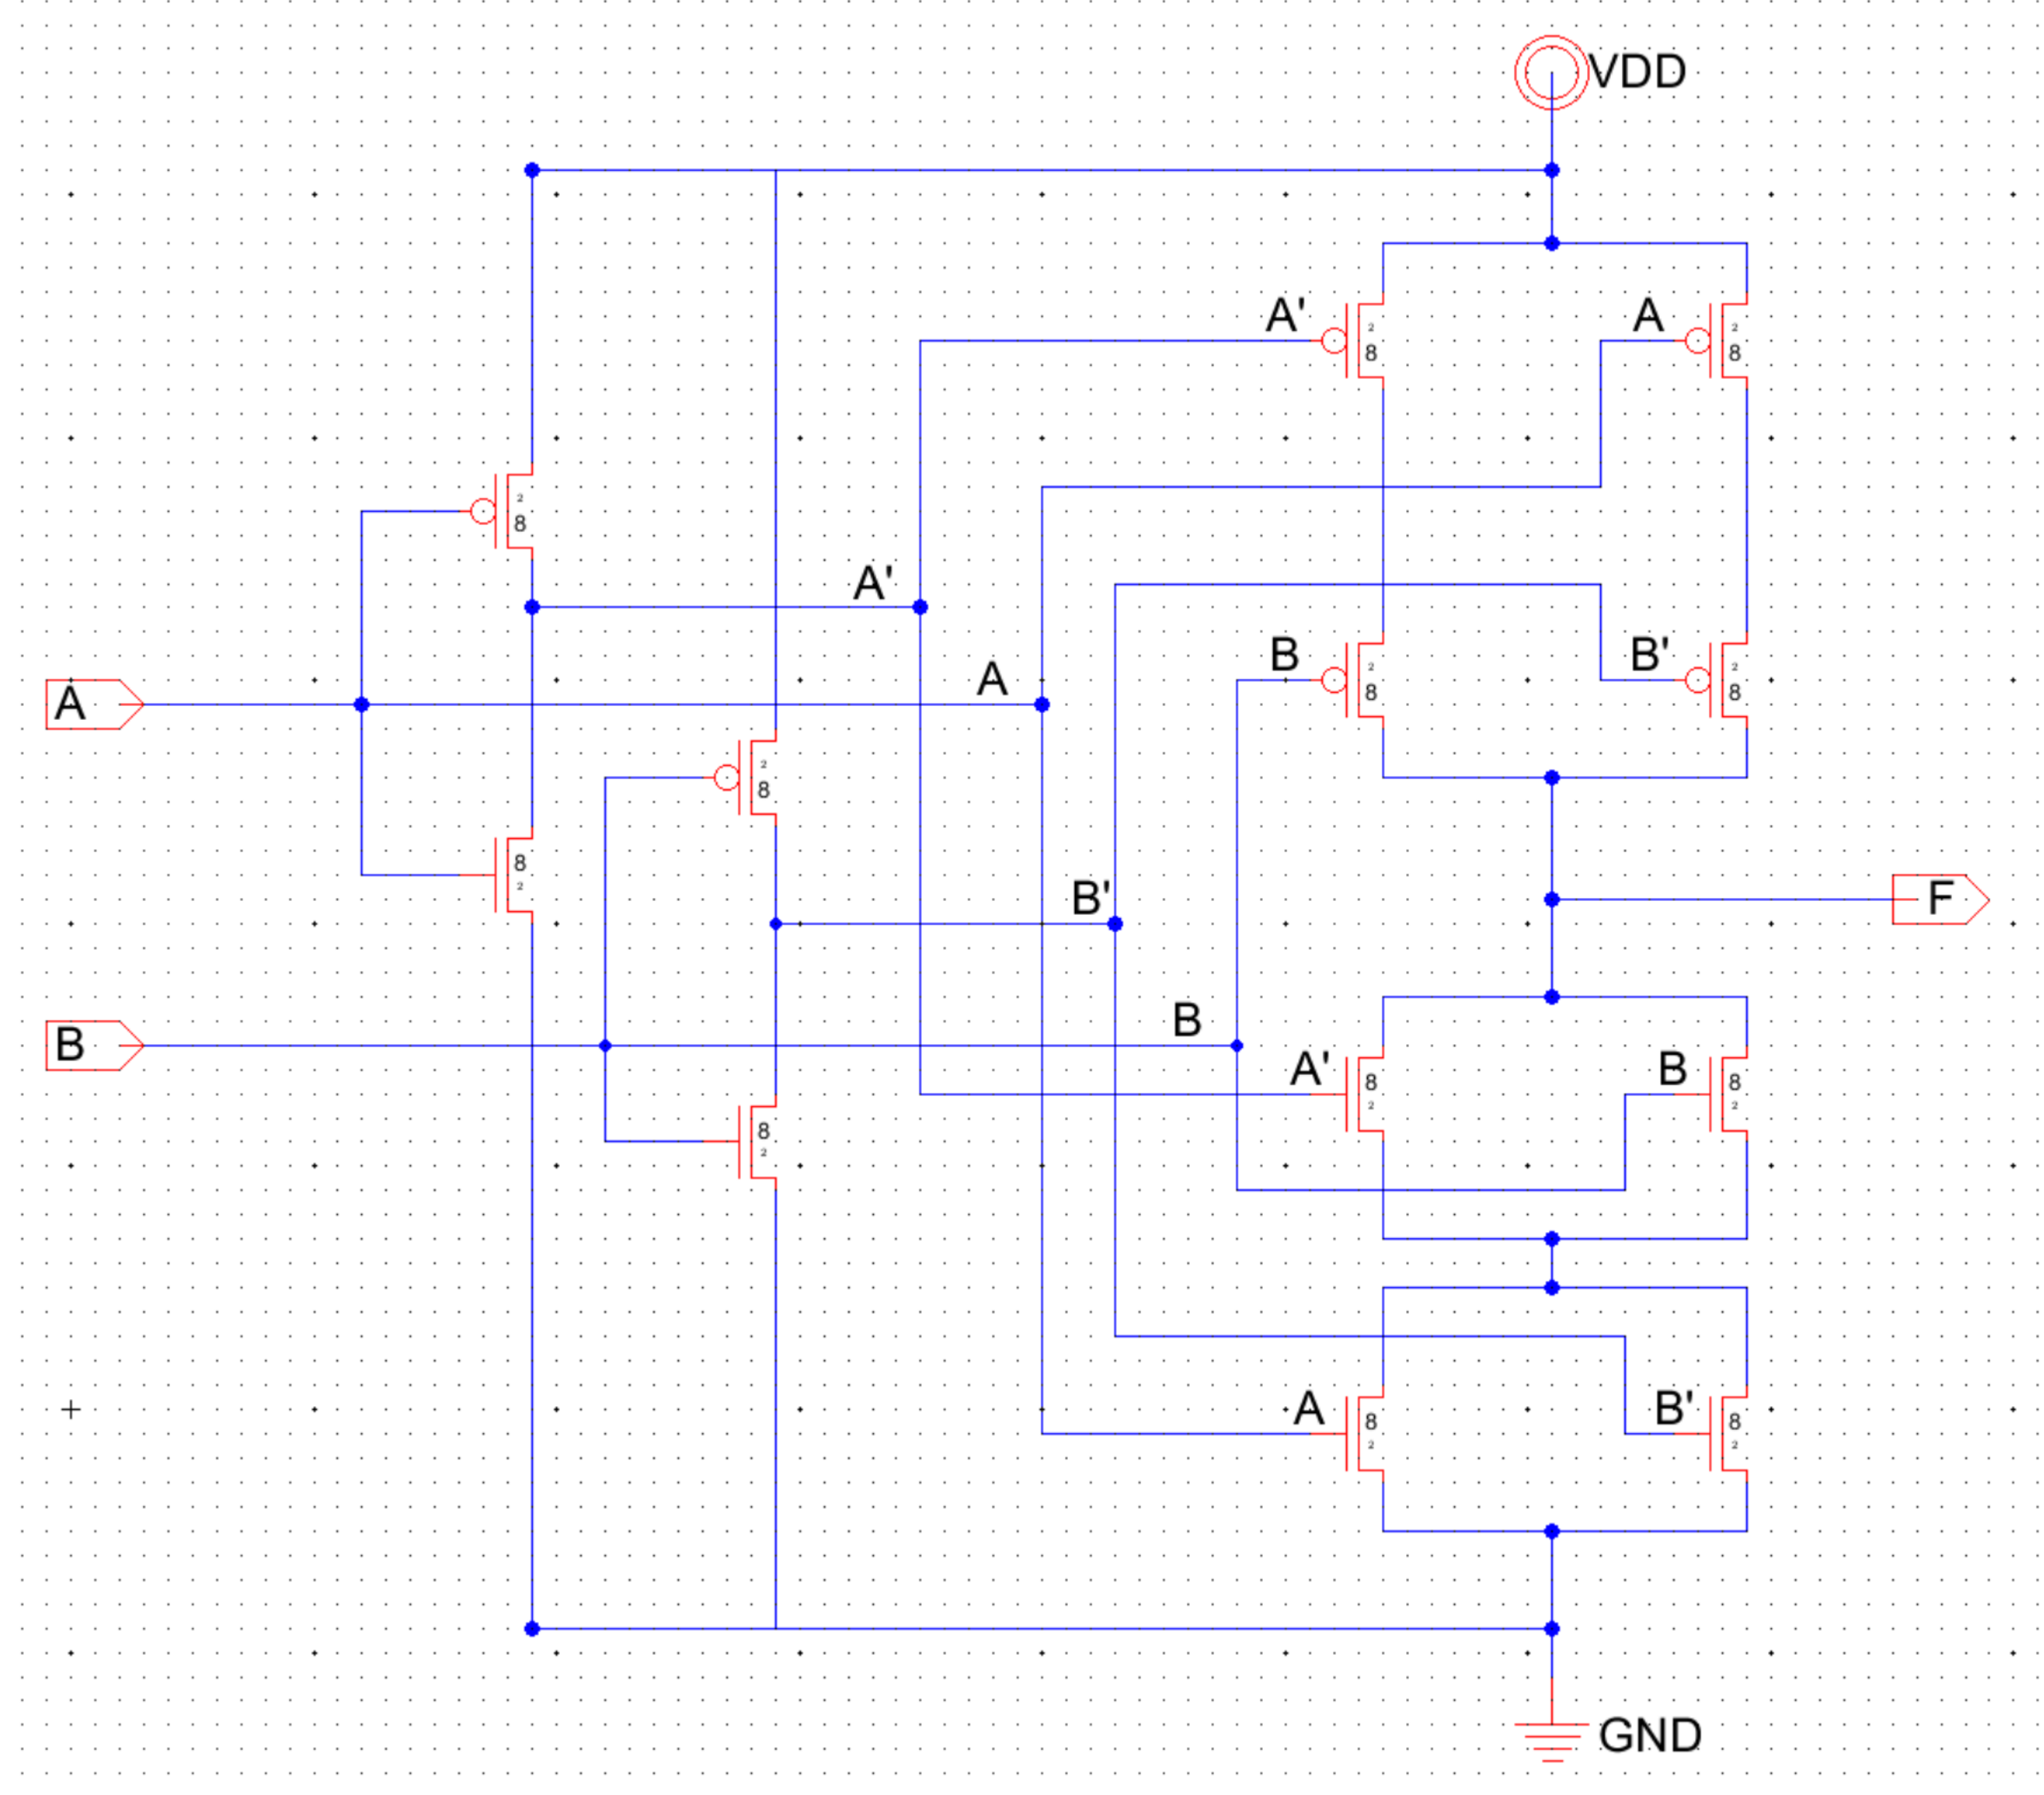
\includegraphics[width=\linewidth, frame]{screenshots/schematic.png}
    \caption{The finished schematic in Electric.}
    \label{fig:schem}
  \end{figure}

  \paragraph{}
  After designing the schematic in electric, it must pass the Design Rule Check (DRC) in order to be simulated properly. The DRC checks to make sure there are no major issues with the schematic. The results of the DRC are shown in Figure \ref{fig:sch-drc}. The DRC has found no errors and the design can be simulated.

  \begin{figure}[H]
    \centering
    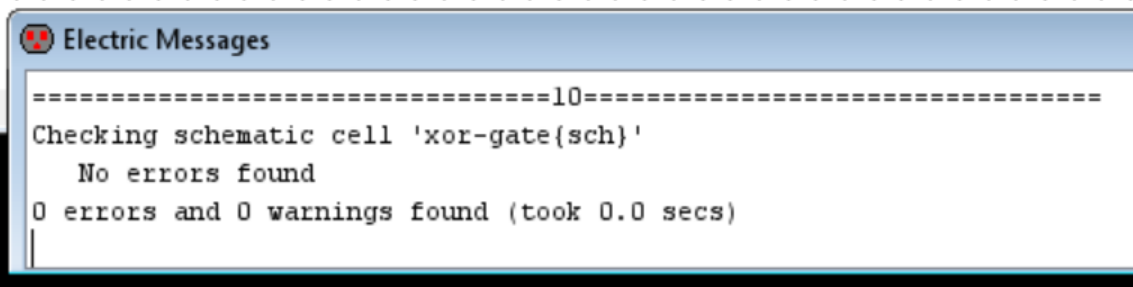
\includegraphics[width=0.9\linewidth, frame]{screenshots/schematic-drc.png}
    \caption{The DRC for the schematic shows no errors.}
    \label{fig:sch-drc}
  \end{figure}

\section{Schematic Simulation}
  \paragraph{}
  The spice code for the simulation of the XOR gate schematic is shown in Figure \ref{fig:spice-sch}. For this simulation, we are required to generate a 2MHz digital signal for input A and a 4MHz digital signal for input B. Both of these signals must have a rise time of 2ns and a fall time of 3ns. This is accomplished with the spice lines \inlinecode{VA A 0 PULSE(3.3 0 0 2n 3n 250n 500n)} for input A and \inlinecode{VB B 0 PULSE(3.3 0 0 2n 3n 125n 250n)} for B. The resulting output signal from these two pulsed input signals can be seen on net F in the simulation graphs.


  \begin{figure}[H]
    \centering
    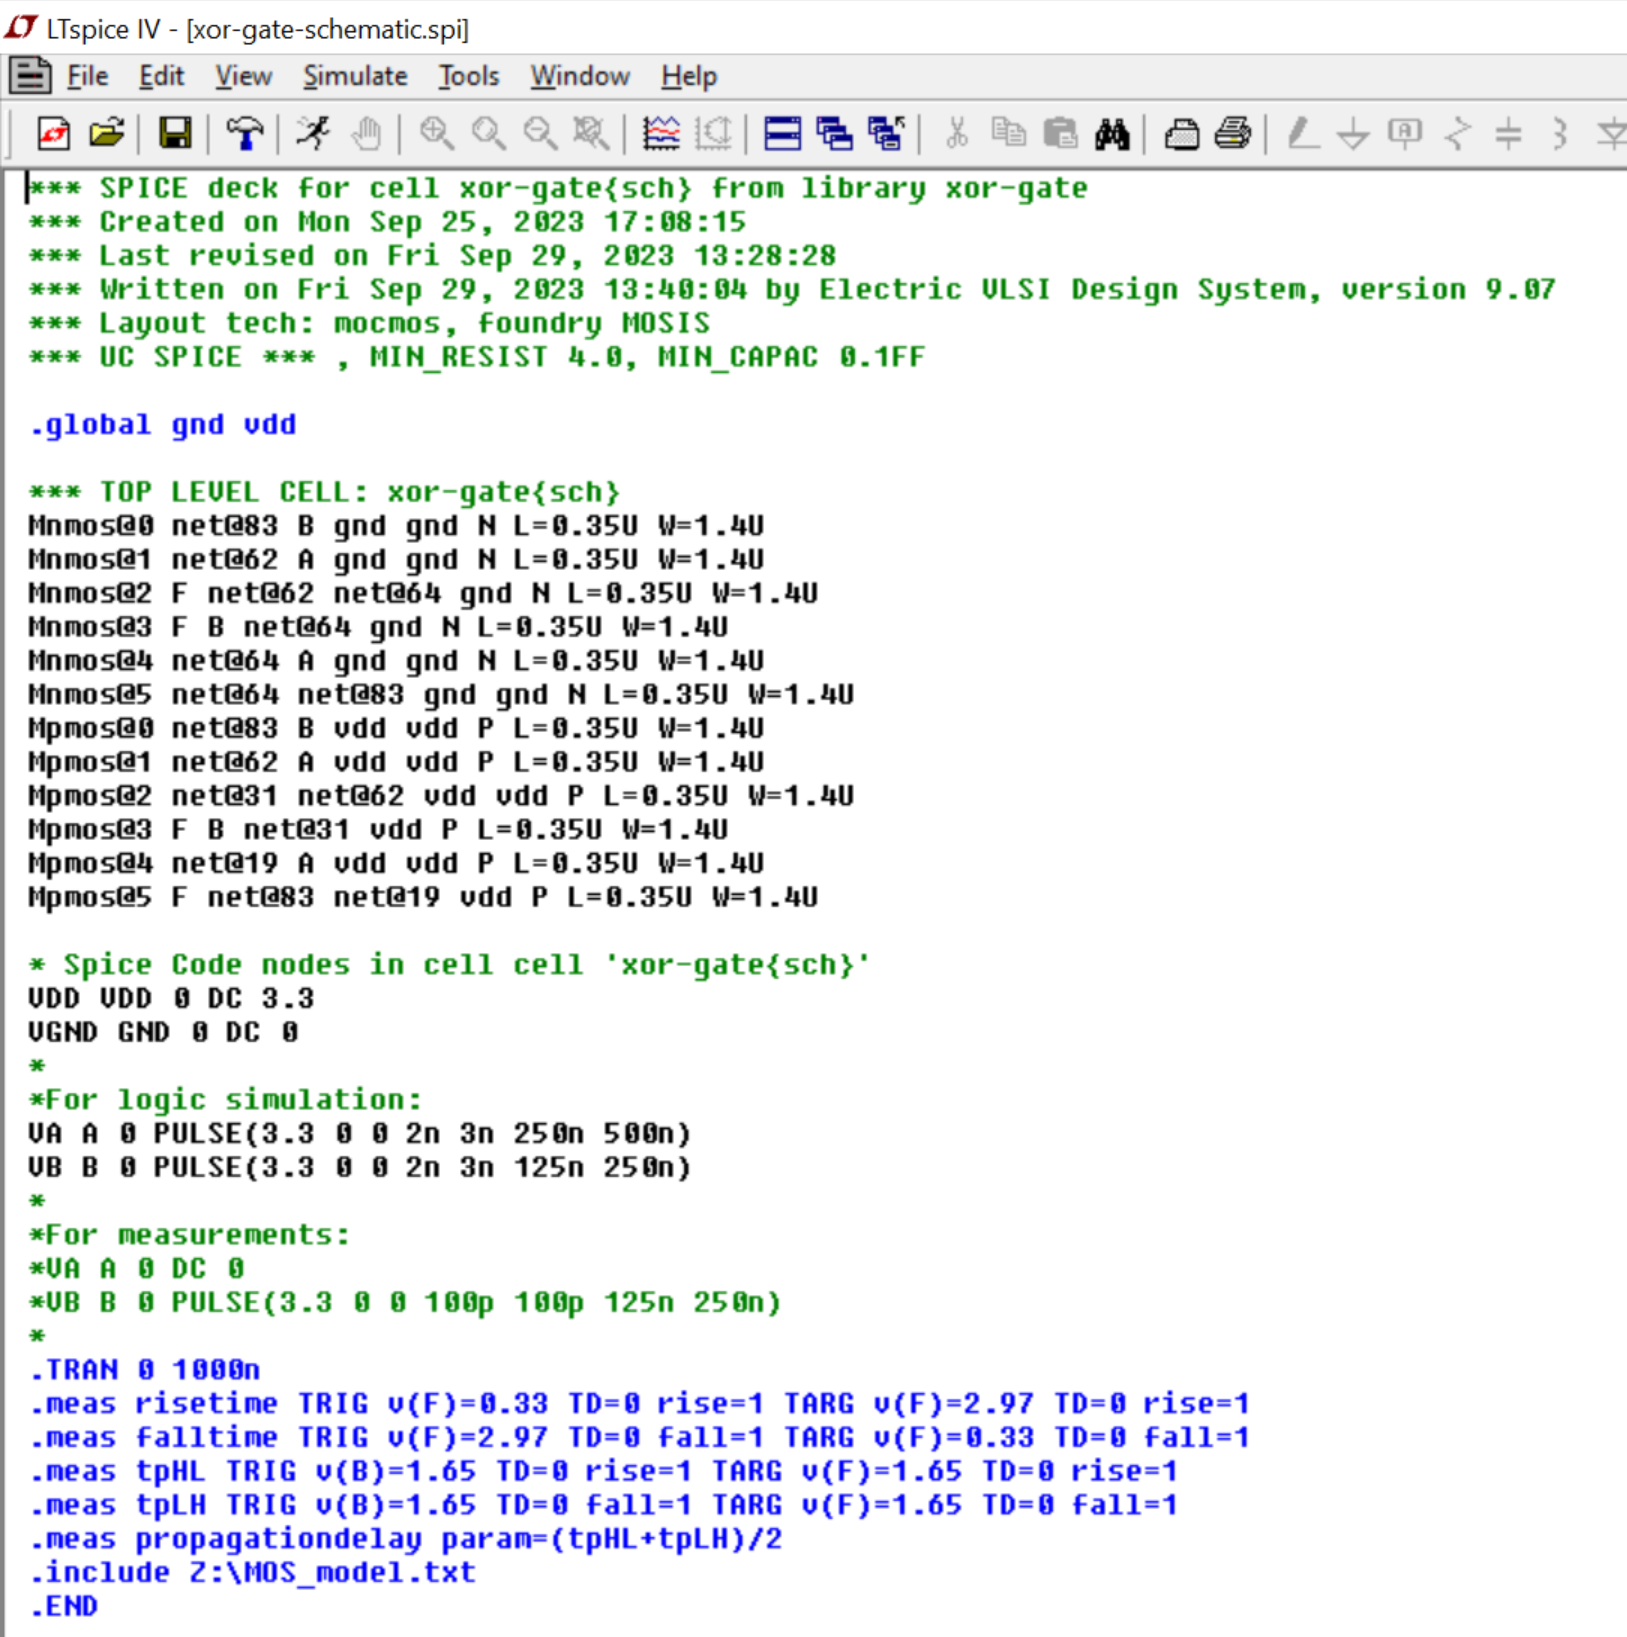
\includegraphics[width=0.9\linewidth, frame]{screenshots/spice-schematic.png}
    \caption{The spice code for simulating the schematic of the XOR gate.}
    \label{fig:spice-sch}
  \end{figure}

  \paragraph{}
  The graphs for the spice simulation of the XOR gate schematic are shown in Figure \ref{fig:sch-sim}. This simulation shows that the schematic is functioning properly since it behaves exactly as we expect an XOR gate to behave. Compare Figure \ref{fig:sch-sim} to Table \ref{table:xor} to see that the functionality is identical.

  \begin{figure}[H]
    \centering
    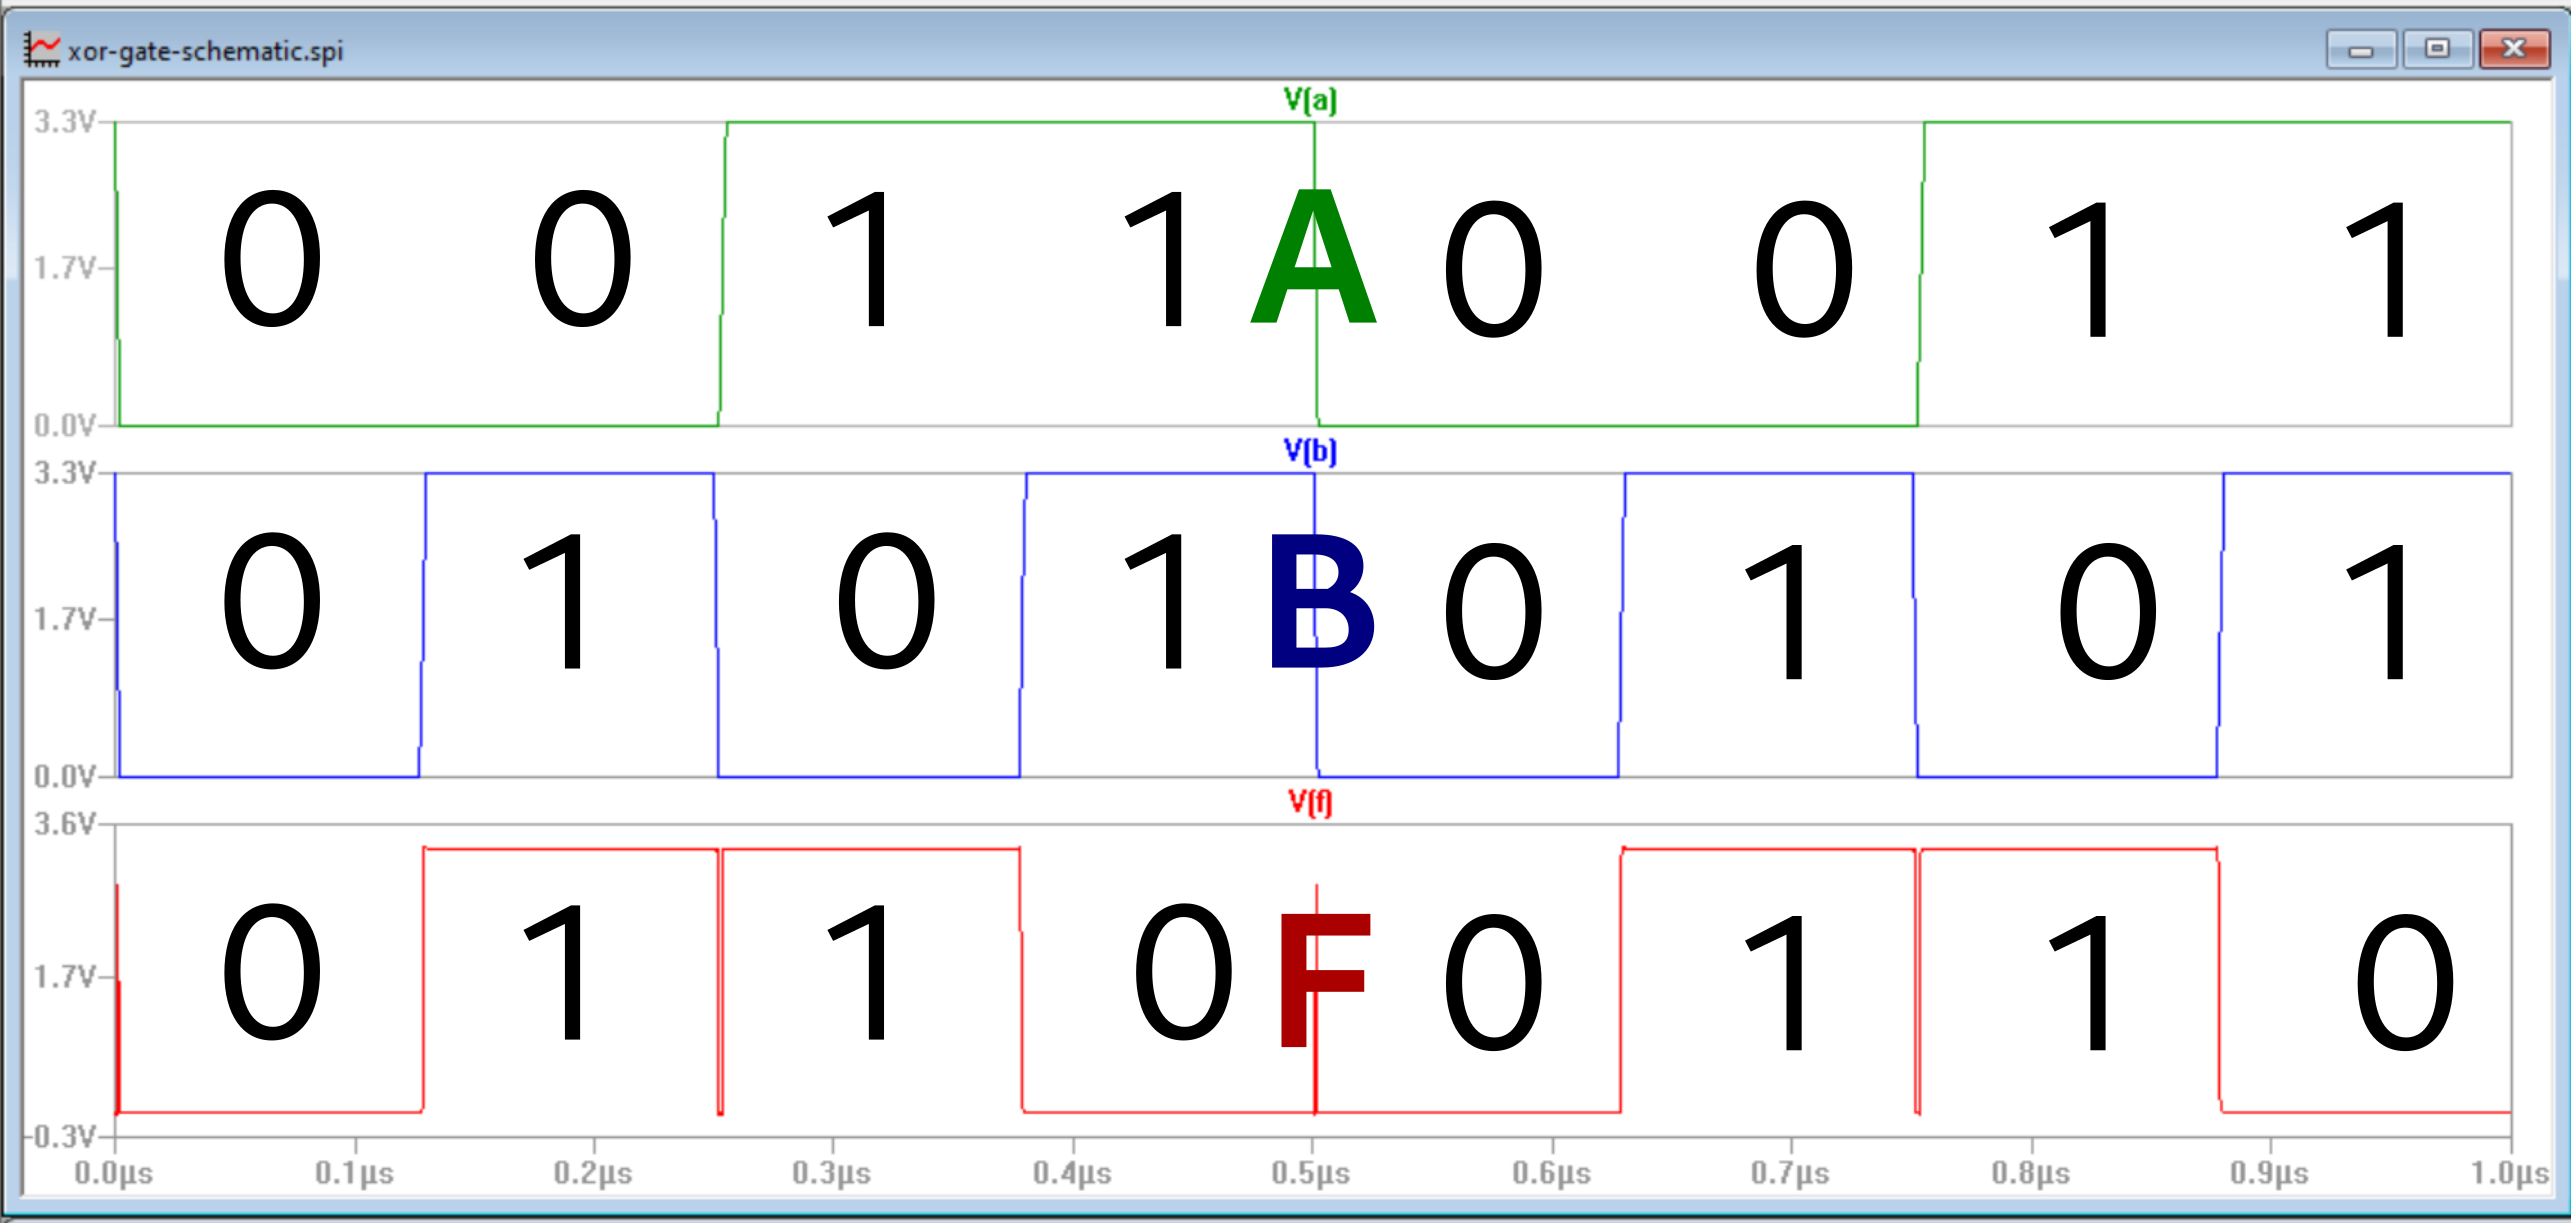
\includegraphics[width=0.9\linewidth, frame]{screenshots/spice-sim-schematic.png}
    \caption{The resulting graphs from the spice simulation of the XOR gate schematic.}
    \label{fig:sch-sim}
  \end{figure}

  \paragraph{}
  IRSIM is different to spice in that its simulation is purely digital. We can use IRSIM to confirm that the behavior of our XOR gate is correct from a purely digital standpoint. IRSIM does not accurately simulate timing like spice does, but is simply another way to validate our design. The rising and falling edges of the inputs must be set manually, and the output at F is automatically shown with each change to the inputs by the user. The resulting graph from the IRSIM simulation of the XOR gate schematic is shown in Figure \ref{fig:irsim-sch}. This simulation shows the correct results that match Figure \ref{fig:sch-sim} and Table \ref{table:xor}.


  \begin{figure}[H]
    \centering
    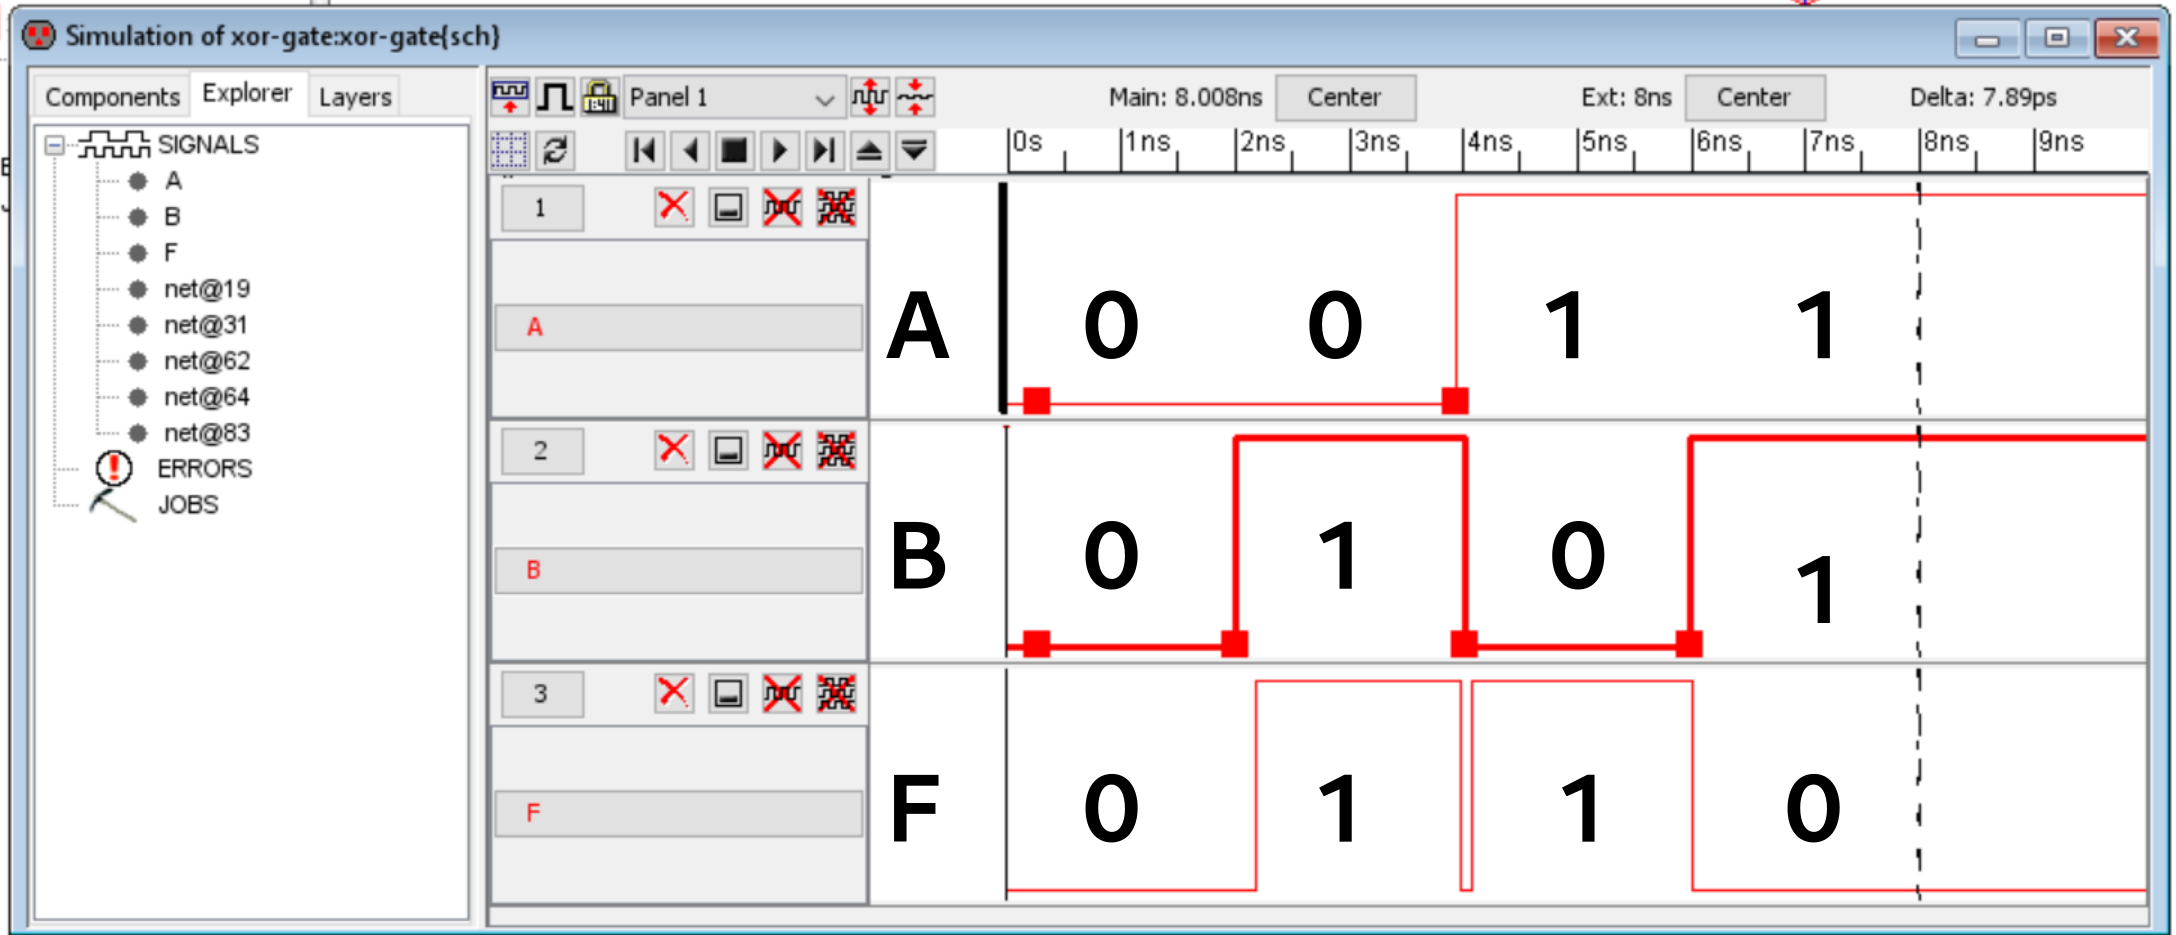
\includegraphics[width=0.9\linewidth, frame]{screenshots/irsim-schematic.png}
    \caption{The resulting graphs from the IRSIM simulation of the XOR gate schematic.}
    \label{fig:irsim-sch}
  \end{figure}

\section{Schematic Measurements}
  \paragraph{}
  We are interested in a number of measurements that give us some indication about the performance of our design. The first measurement we are concerned with is the Rise Time of the output signal. The Rise Time of a signal is the amount of time it takes for the signal to go from 10\% of VDD to 90\% of VDD on a rising edge. A rise time that is too slow can cause issues with the propogation of the signal through a system. Similarly, the Fall Time is the time it takes for a signal to go from 90\% of VDD to 10\% of VDD on the falling edge. It is also important that the fall time be fast enough. 

  \paragraph{}
  Another important metric is the propagation delay. $t_{pHL}$ is a measure of the time between when the rising edge of the input signal hits 50\% of VDD and when the falling edge of the output signal hits 50\% of VDD. It essentially tells us the time for a rising edge to propagate from input to falling edge of the output. Similarly, $t_{pLH}$ is the time from falling edge of the input to rising edge of the output (also measured from 50\% of VDD for each). The propagation delay is then the average of the two, as in $Propagation\ Delay=\frac{t_{pHL}+t_{pLH}}{2}$.

  \paragraph{}
  The spice code for measuring these parameters is shown in Figure \ref{fig:sch-sim-meas}. The first thing to note is that input A is kept at a constant 3.3V so that we can pulse input B and get the inverse waveform at output F. The rise and fall times were also modified from 2ns and 3ns to 100ps. I found that the 2ns and 3ns rise and fall times were too slow, and as a result the output signal would actually reach 50\% of VDD before the input signal did. Changing the rise and fall times to 100ps solved this issue and allowed me to take accurate measurements. 

  \begin{figure}[H]
    \centering
    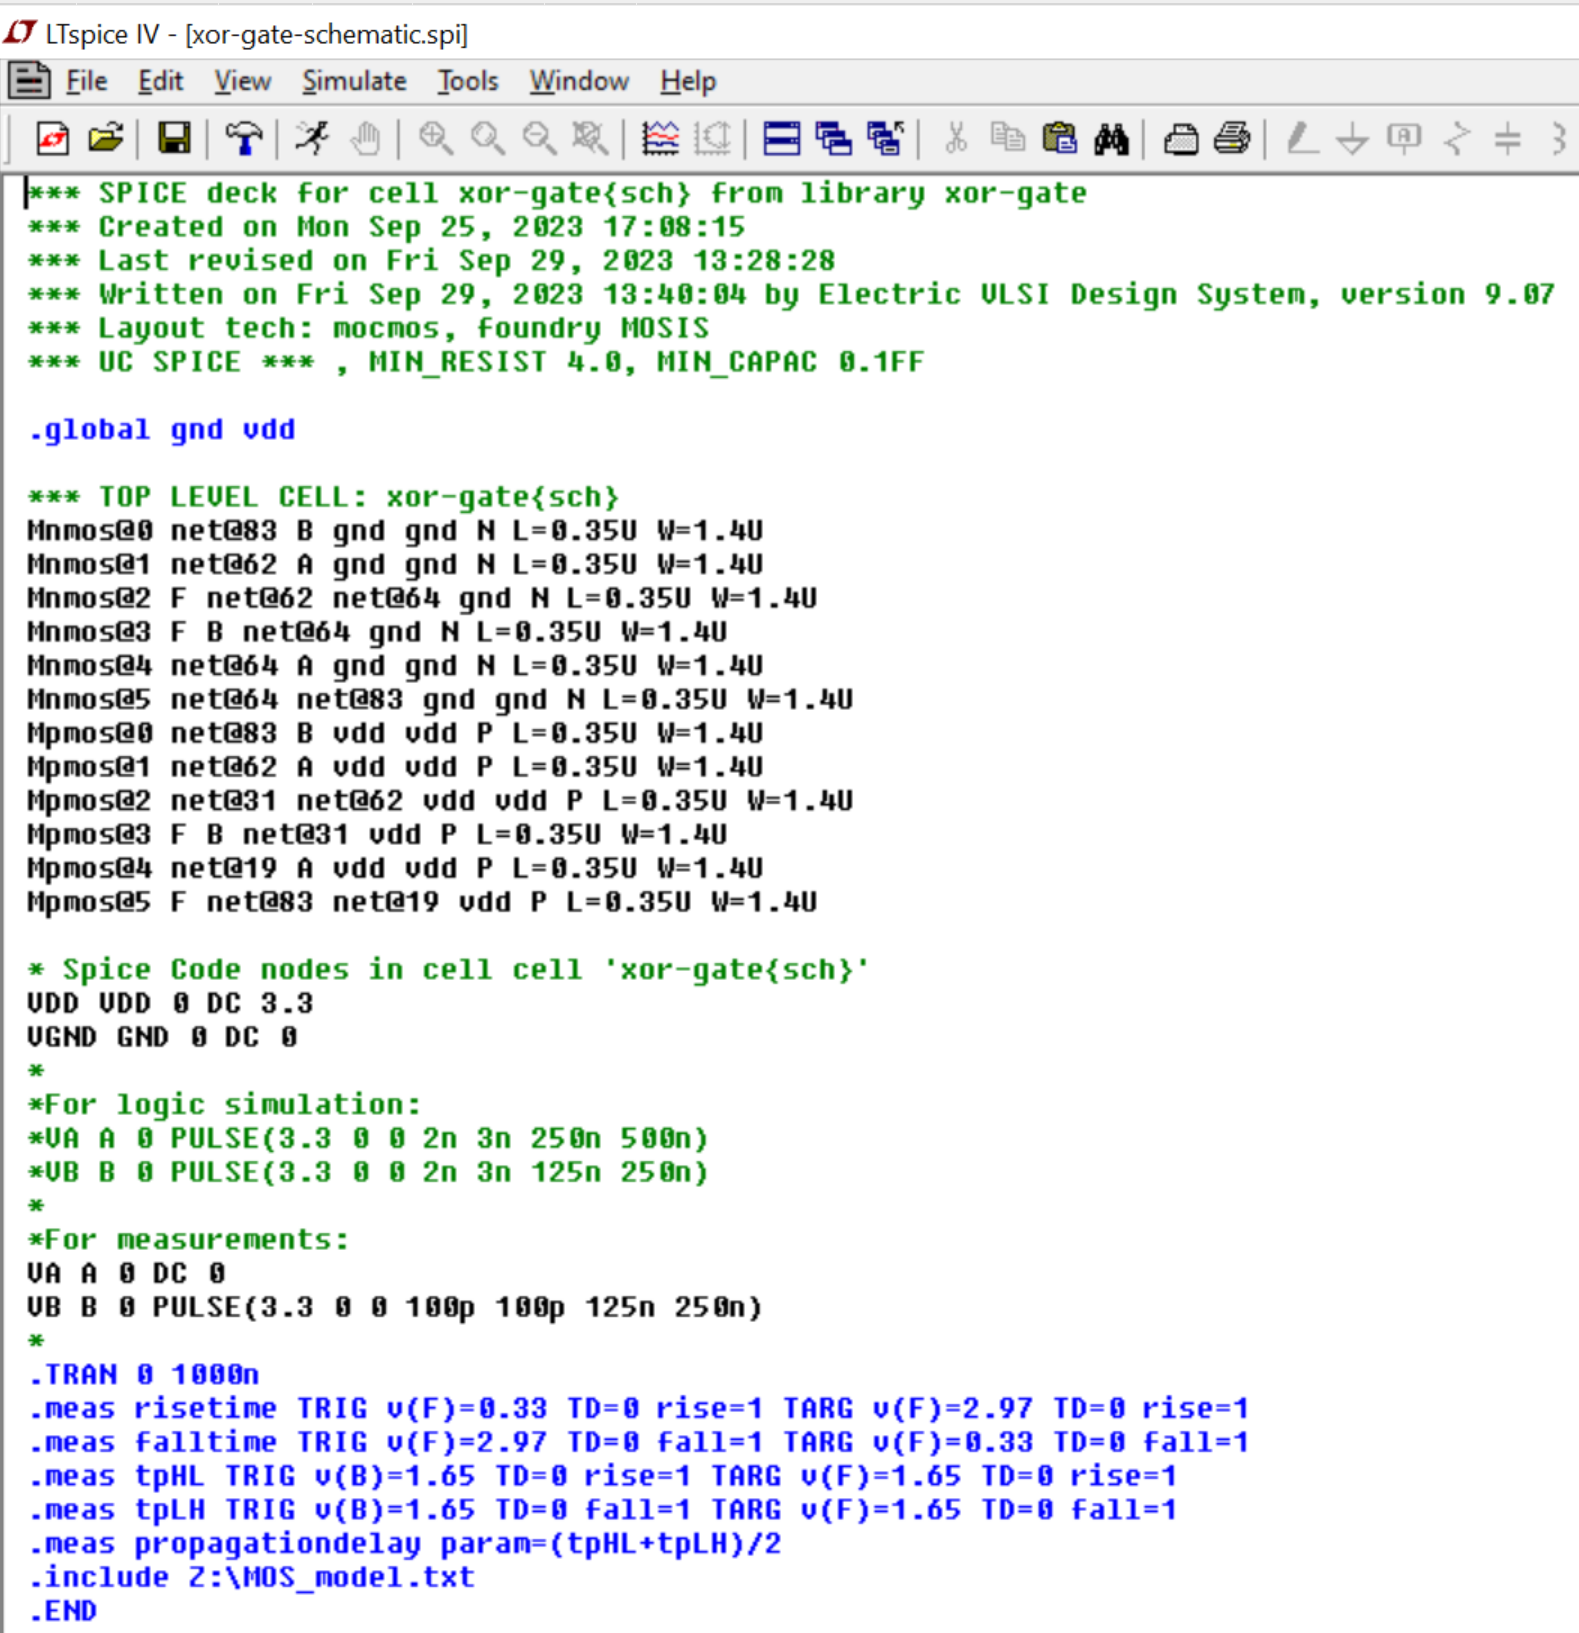
\includegraphics[width=0.9\linewidth, frame]{screenshots/spice-meas-schematic.png}
    \caption{The spice code that measures the rise time, fall time, and propagation delay of the output signal of the XOR gate schematic.}
    \label{fig:sch-sim-meas}
  \end{figure}

  \paragraph{}
  The lines of spice code that start with \inlinecode{.meas} are the lines that actually take the measurements we are interested in. The line \inlinecode{.meas risetime TRIG v(F)=0.33 TD=0 rise=1 TARG v(F)=2.97 TD=0 rise=1} calculates the rise time by recording the time when output F reaches 10\% of VDD and the time when F reaches 90\% of VDD and then finding the difference. Similarly, the line \inlinecode{.meas falltime TRIG v(F)=2.97 TD=0 fall=1 TARG v(F)=0.33 TD=0 fall=1} measures the fall time by determining the length of time between F reaching 90\% of VDD and it reaching 10\% of VDD. The line \inlinecode{.meas tpHL TRIG v(B)=1.65 TD=0 rise=1 TARG v(F)=1.65 TD=0 fall=1} measures $t_{pHL}$ by finding the time between the 50\% point of the rising edge of input B and the 50\% point of the falling edge of output F. The line \inlinecode{.meas tpLH TRIG v(B)=1.65 TD=0 fall=1 TARG v(F)=1.65 TD=0 rise=1} does the same except it measures from the falling edge of B and the rising edge of F in order to measure $t_{pLH}$. Finally, the line \inlinecode{.meas propagationdelay param=(tpHL+tpLH)/2} averages $t_{pHL}$ and $t_{pLH}$ in order to calculate the propagation delay.

  \paragraph{}
  After running the code in LTSpice, the measurements can be viewed by opening the error log. The results of these measurements are shown in Figure \ref{fig:meas-sch}. The measurements can be viewed more clearly in Table \ref{table:meas-sch}.

  \begin{figure}[H]
    \centering
    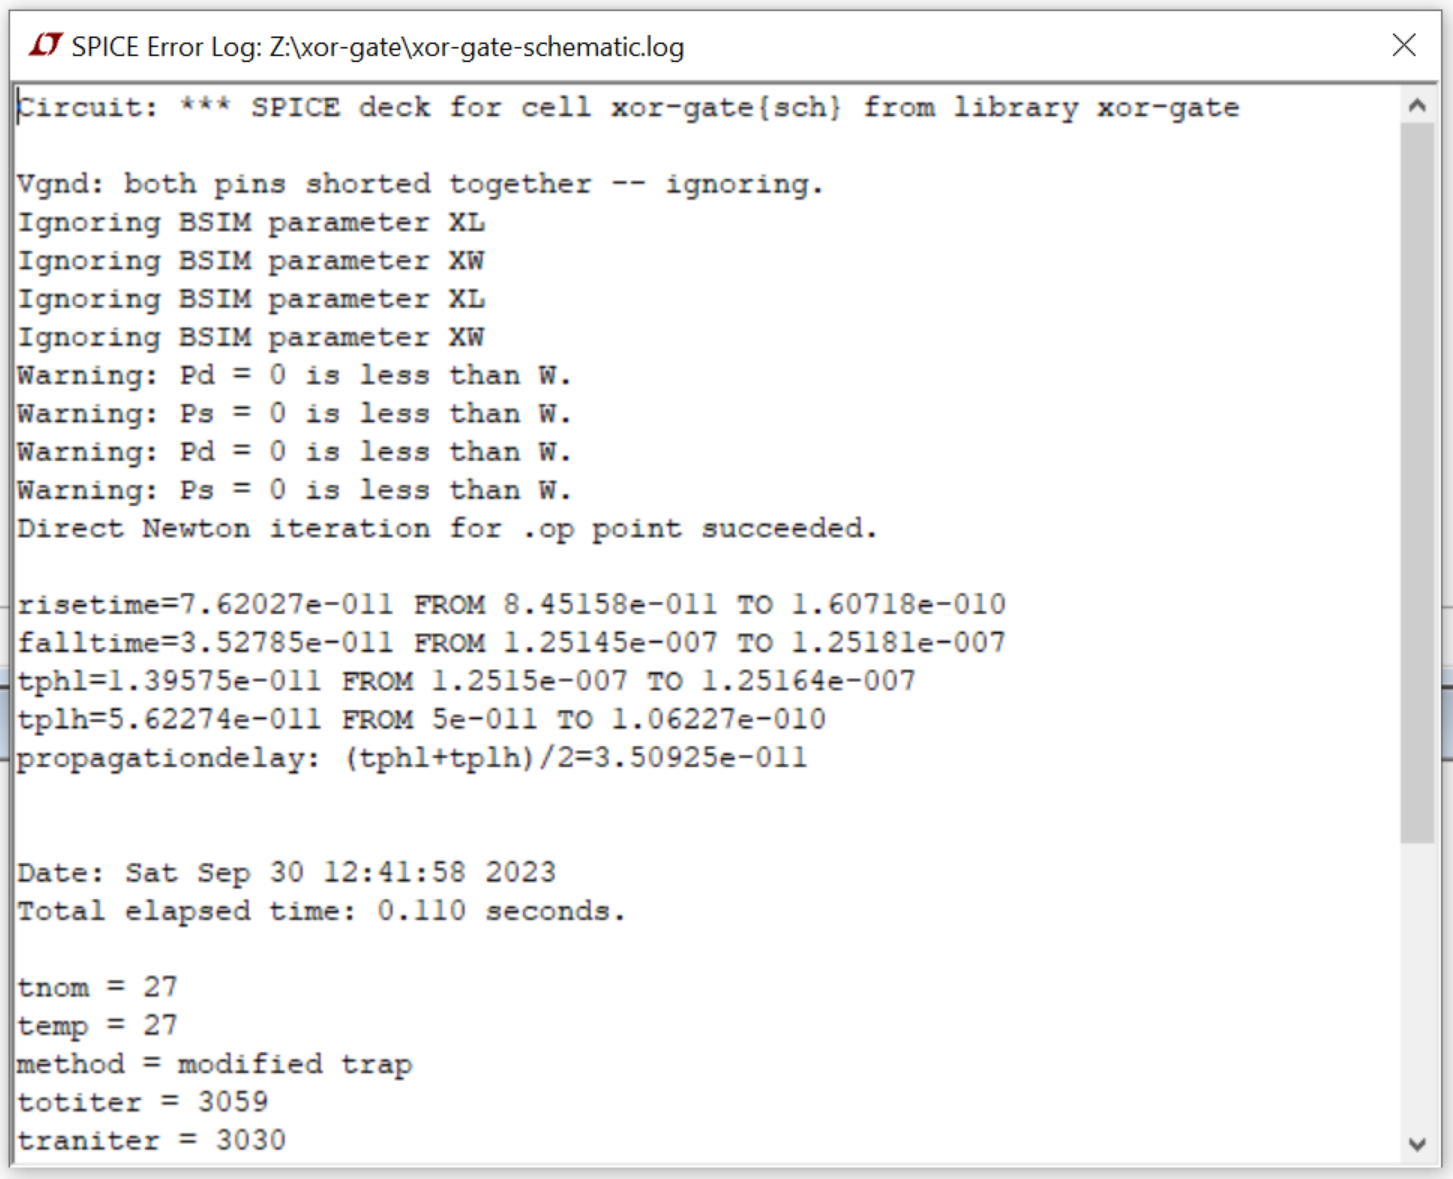
\includegraphics[width=0.7\linewidth, frame]{screenshots/meas-schematic.png}
    \caption{The output from LTSpice showing the measurements done on the output of the XOR gate schematic.}
    \label{fig:meas-sch}
  \end{figure}


  \begin{table}[H]
    \centering
    \footnotesize
    \begin{tabular}{|c|c|}
      \hline
      \textbf{Parameter} & \textbf{Measurement} \\
      \hline
      Rise Time & 76.2ps\\
      \hline
      Fall Time & 35.3ps \\
      \hline
      $t_{pHL}$ & 14.0ps \\
      \hline
      $t_{pLH}$ & 56.2ps \\
      \hline
      Propagation Delay & 35.1ps \\
      \hline
    \end{tabular}
    \caption{The measurements done on the XOR gate schematic in LTSpice.}
    \label{table:meas-sch}
  \end{table}


\section{Layout in Electric}
  \paragraph{}
  I began designing the layout with a stick diagram, as shown in Figure \ref{fig:stick}. I started with the active areas and then drew the polysilicon gates. I planned out which gates would take which input signal by looking at the various nodes of the schematic in Figure \ref{fig:schem} and determining which transistors from the schematic should be adjacent. Then I routed the metal layer to connect the transistor sources and drains to each other and to VDD and GND. Finally, I added the inverters to the left and routed $A$, $B$, $\overline{A}$, and $\overline{B}$ to the proper transistor pairs on the right.


  \begin{figure}[H]
    \centering
    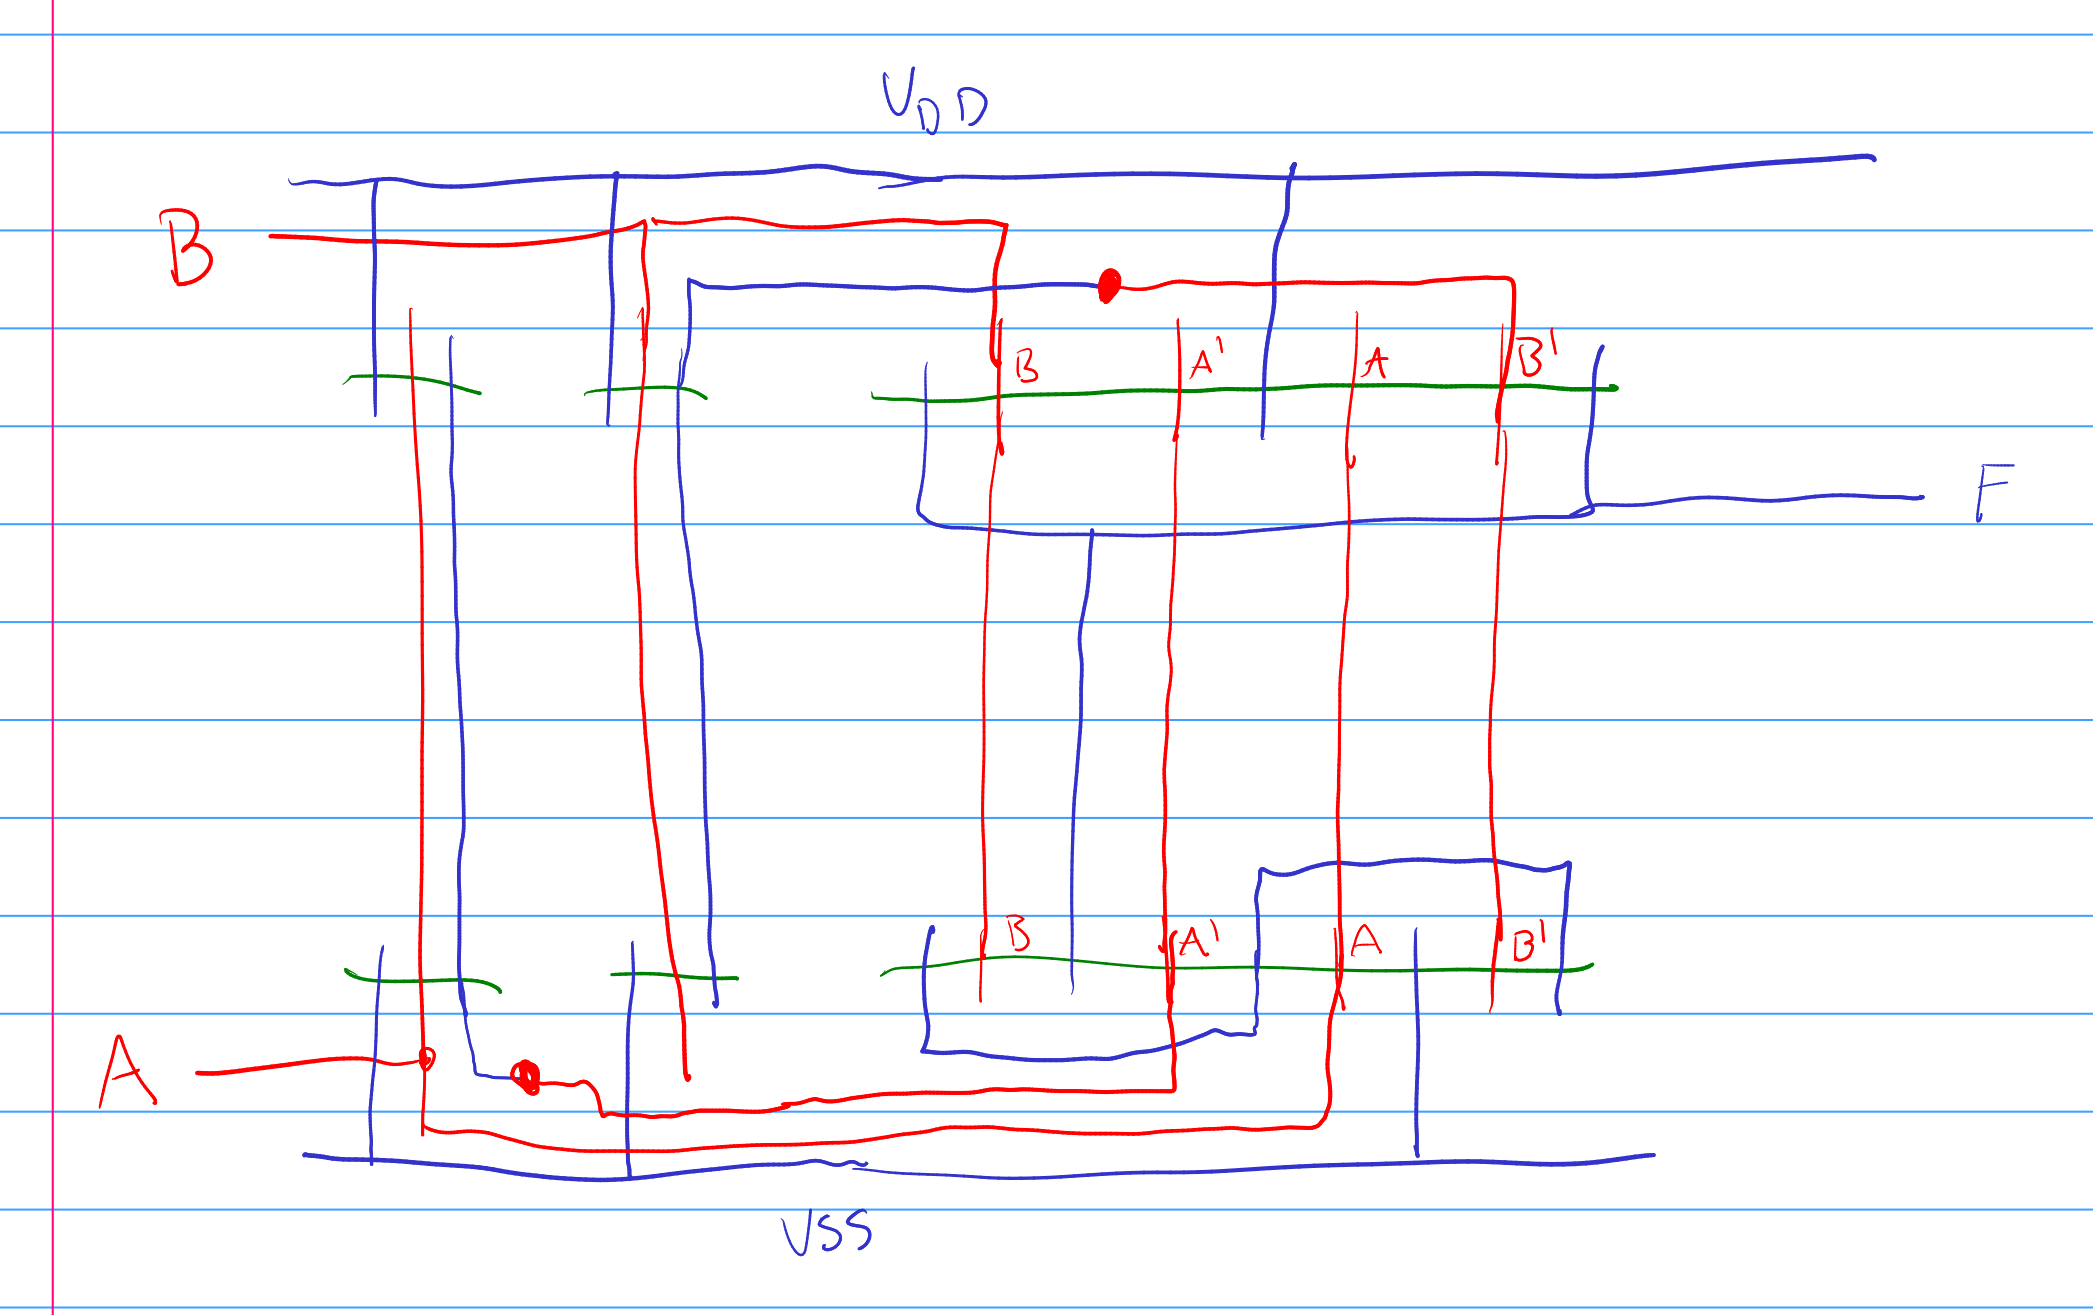
\includegraphics[width=0.7\linewidth, frame]{screenshots/stick-diagram.png}
    \caption{The stick diagram used to plan out the layout of the XOR gate.}
    \label{fig:stick}
  \end{figure}

  \paragraph{}
  I then turned the stick diagram into the layout in Figure \ref{fig:layout} with some minor changes to optimize space. For instance, $A$ is now on top on the input side and there is a much more direct connection from $B$ at the input of the inverter to the input to the right of the inverter. Both of these changes save space. The spacing of every part of the design is as close as possible while still passing the DRC. The VDD and GND wells may look like they can be closer, but the metal to polysilicon contacts are in the way and there is nowhere else to place them. It may be noted that the NMOS transistors of the inverters are shifted up slightly - this is to allow me to place GND closer to the rest of the design. I would move the NMOS transistors from the PDN up as well, but that would cause the metal traces to be too close together to pass the DRC. As far as I am aware, every space between design elements has been minimized. The design also conforms to design rules discussed in class that are not built into Electric's design rules, such as the 3$\lambda$ wide rule for the metal layer.


  \begin{figure}[H]
    \centering
    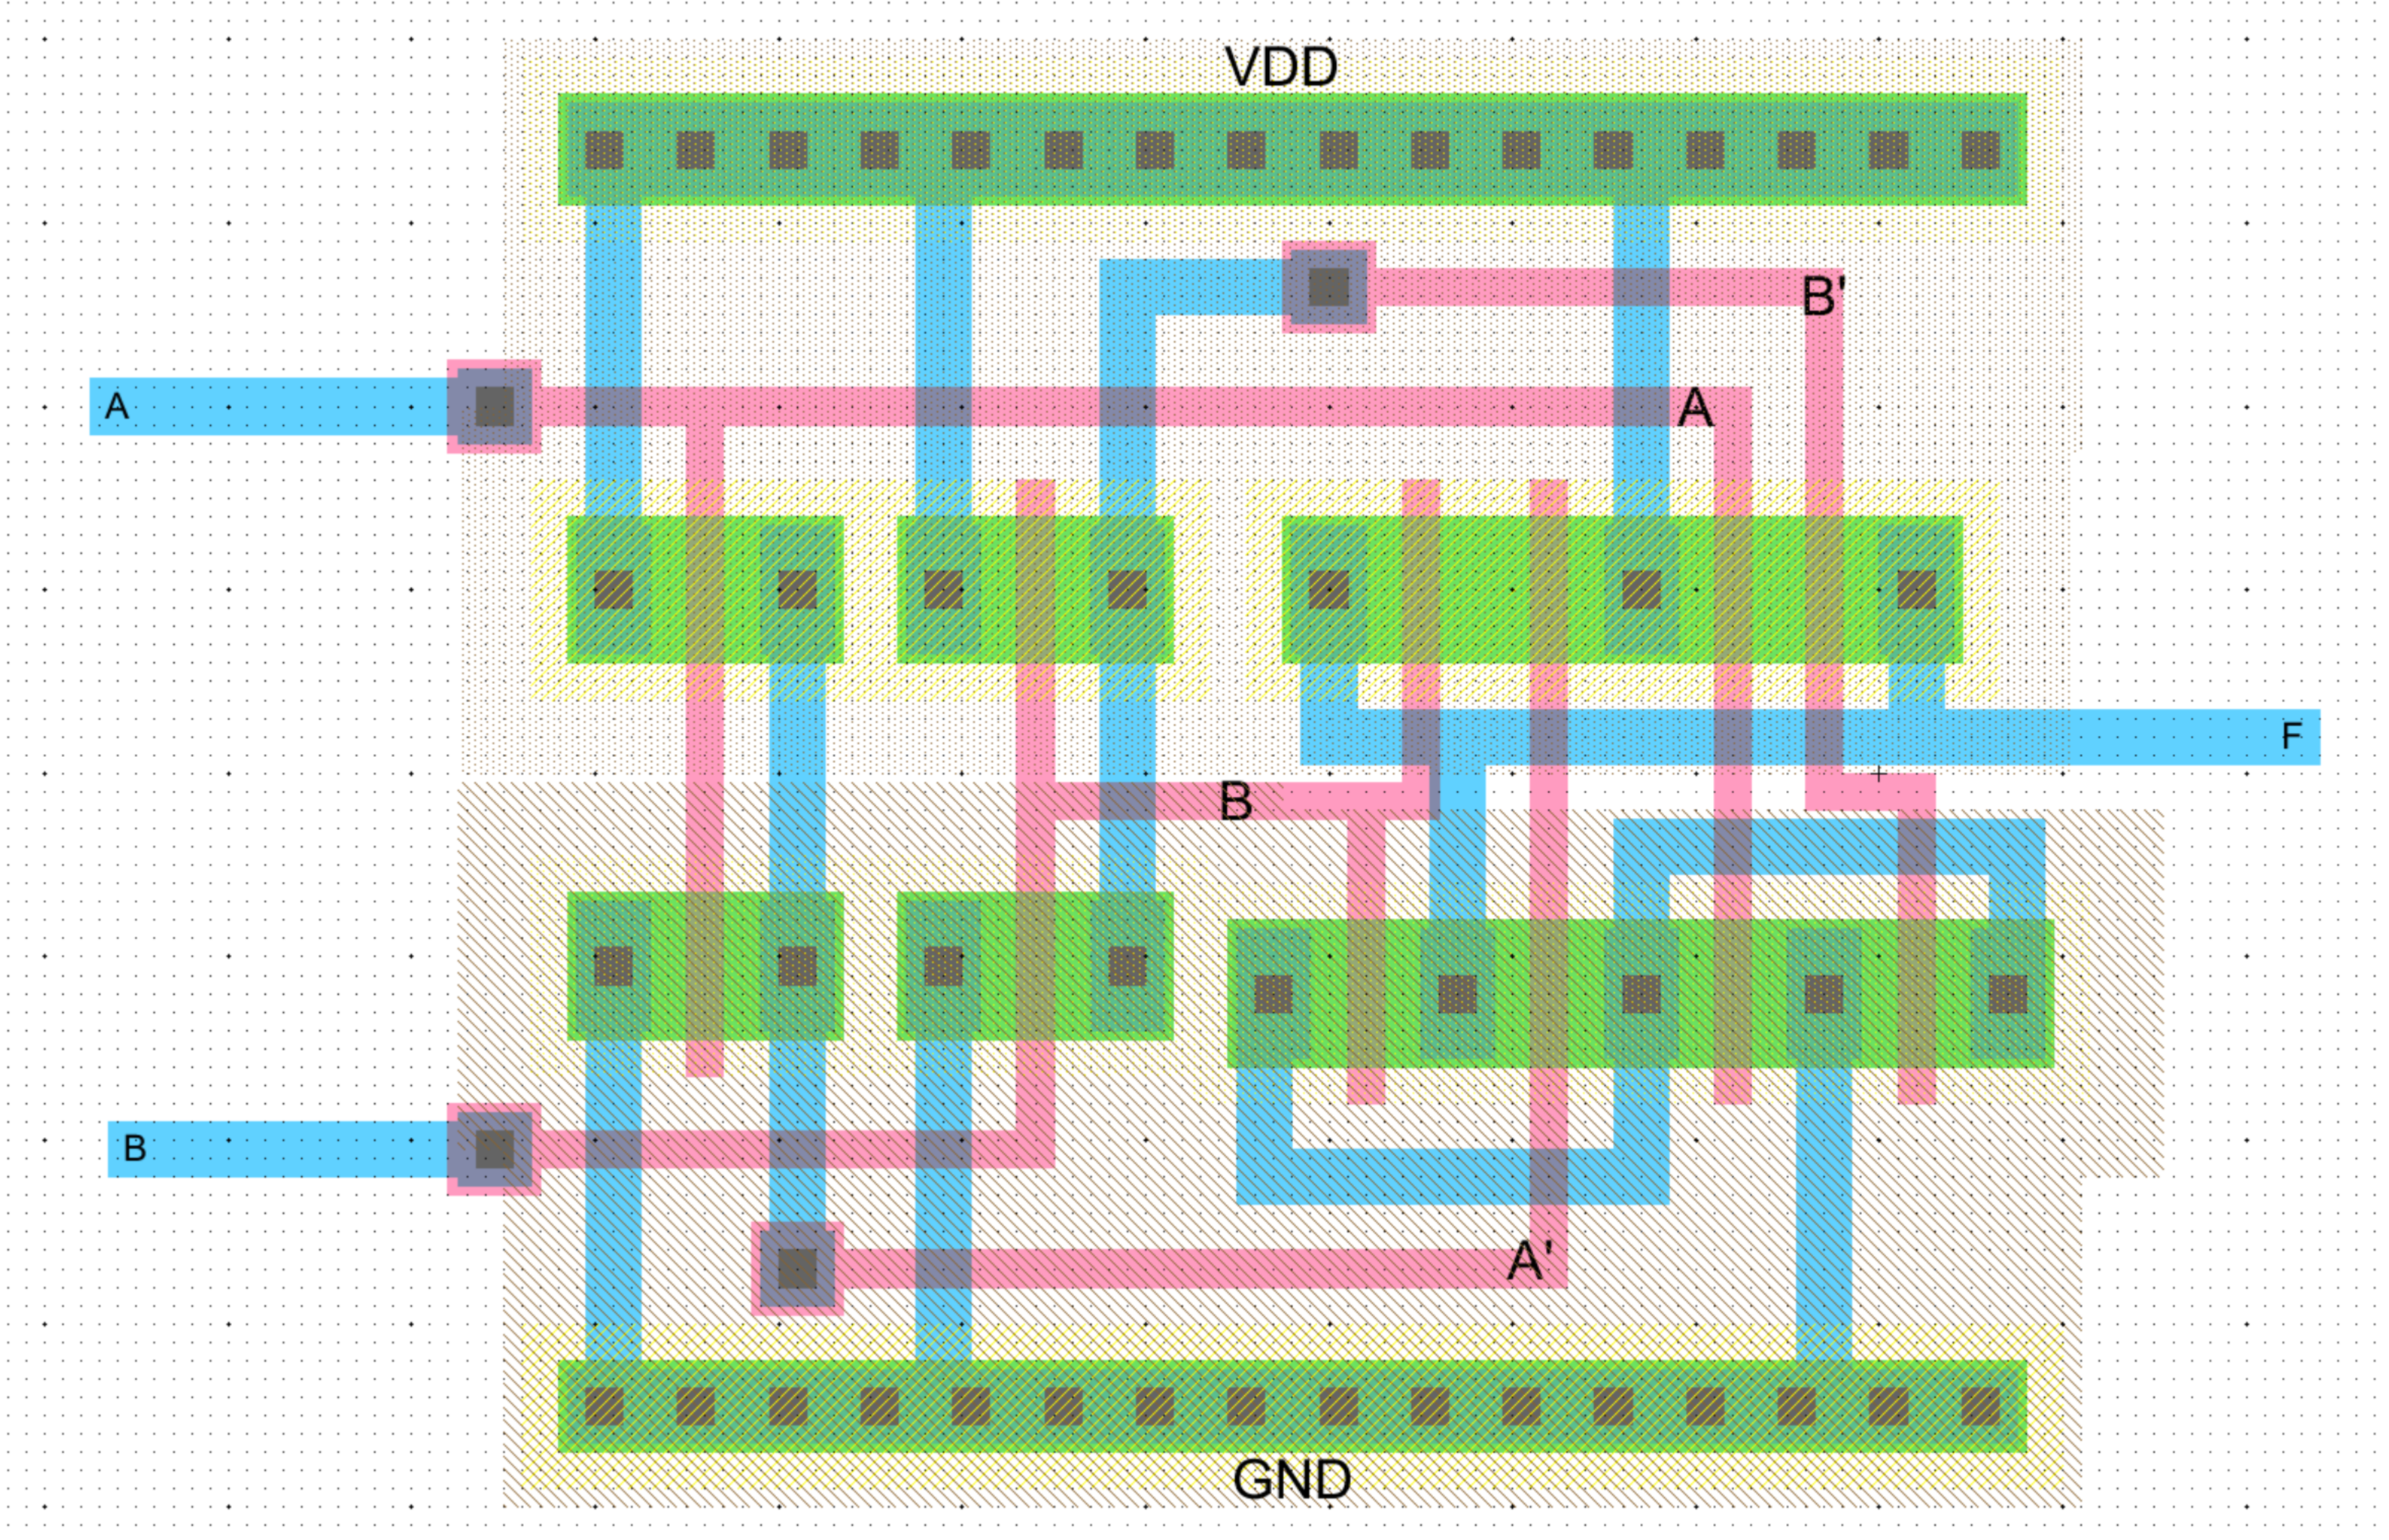
\includegraphics[width=\linewidth, frame]{screenshots/layout.png}
    \caption{The layout of the XOR gate in Electric.}
    \label{fig:layout}
  \end{figure}

  \paragraph{}
  For the layout, the DRC is very important, since it specifies rules for distances between, widths of, and lengths of parts of the design that must be met. These rules ensure that the design is both functional and able to be manufactured. The results of the DRC check for the XOR gate layout are shown in figure \ref{fig:lay-drc}. The design passes the DRC check. It is also important to do a well check (which is in the ERC tools in Electric) to ensure that wells that should be connected are. The results of this check are shown in Figure \ref{fig:well-check}, which shows no errors.


  \begin{figure}[H]
    \centering
    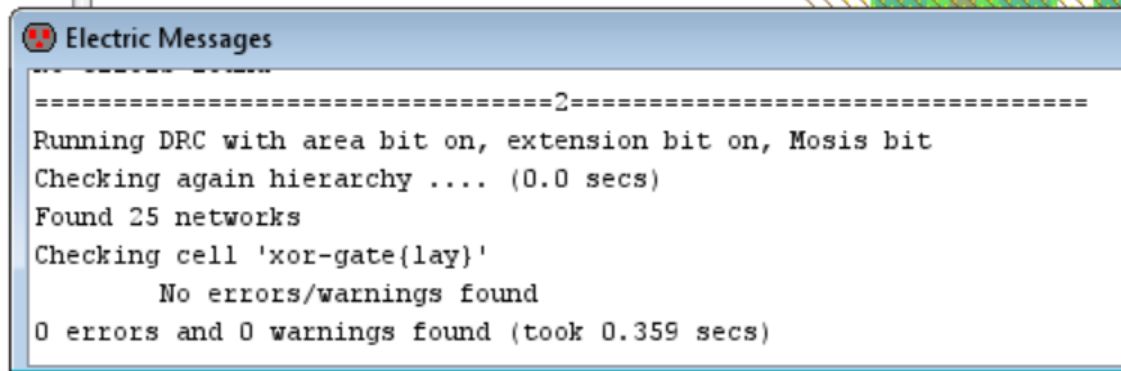
\includegraphics[width=0.7\linewidth, frame]{screenshots/layout-drc.png}
    \caption{The DRC results for the XOR gate layout showing no errors.}
    \label{fig:lay-drc}
  \end{figure}


  \begin{figure}[H]
    \centering
    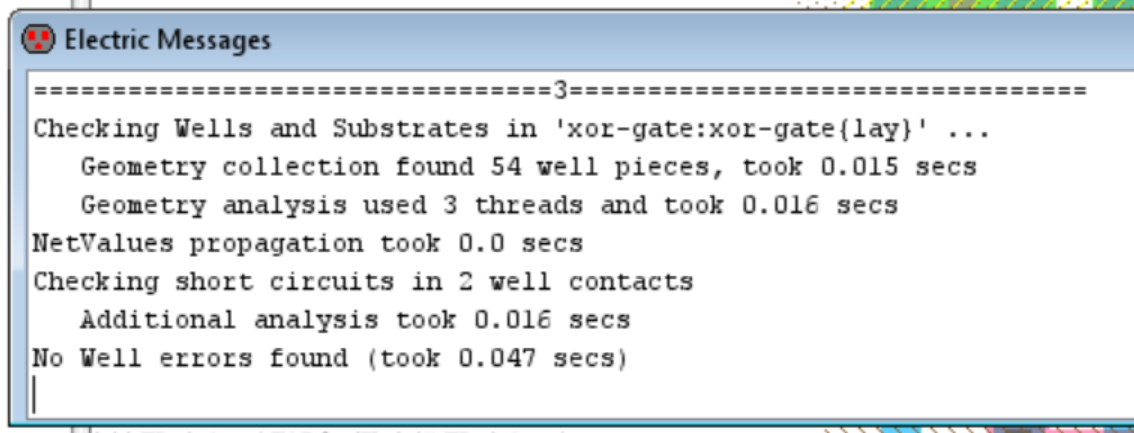
\includegraphics[width=0.7\linewidth, frame]{screenshots/layout-well-check.png}
    \caption{The well check results for the XOR gate layout showing no errors.}
    \label{fig:well-check}
  \end{figure}

\section{Layout Simulation}
  \paragraph{}
  The process for simulating the layout in LTSpice is essentially the same as for the simulation of the schematic. The spice code for the simulation can be seen in Figure \ref{fig:spice-lay}.


  \begin{figure}[H]
    \centering
    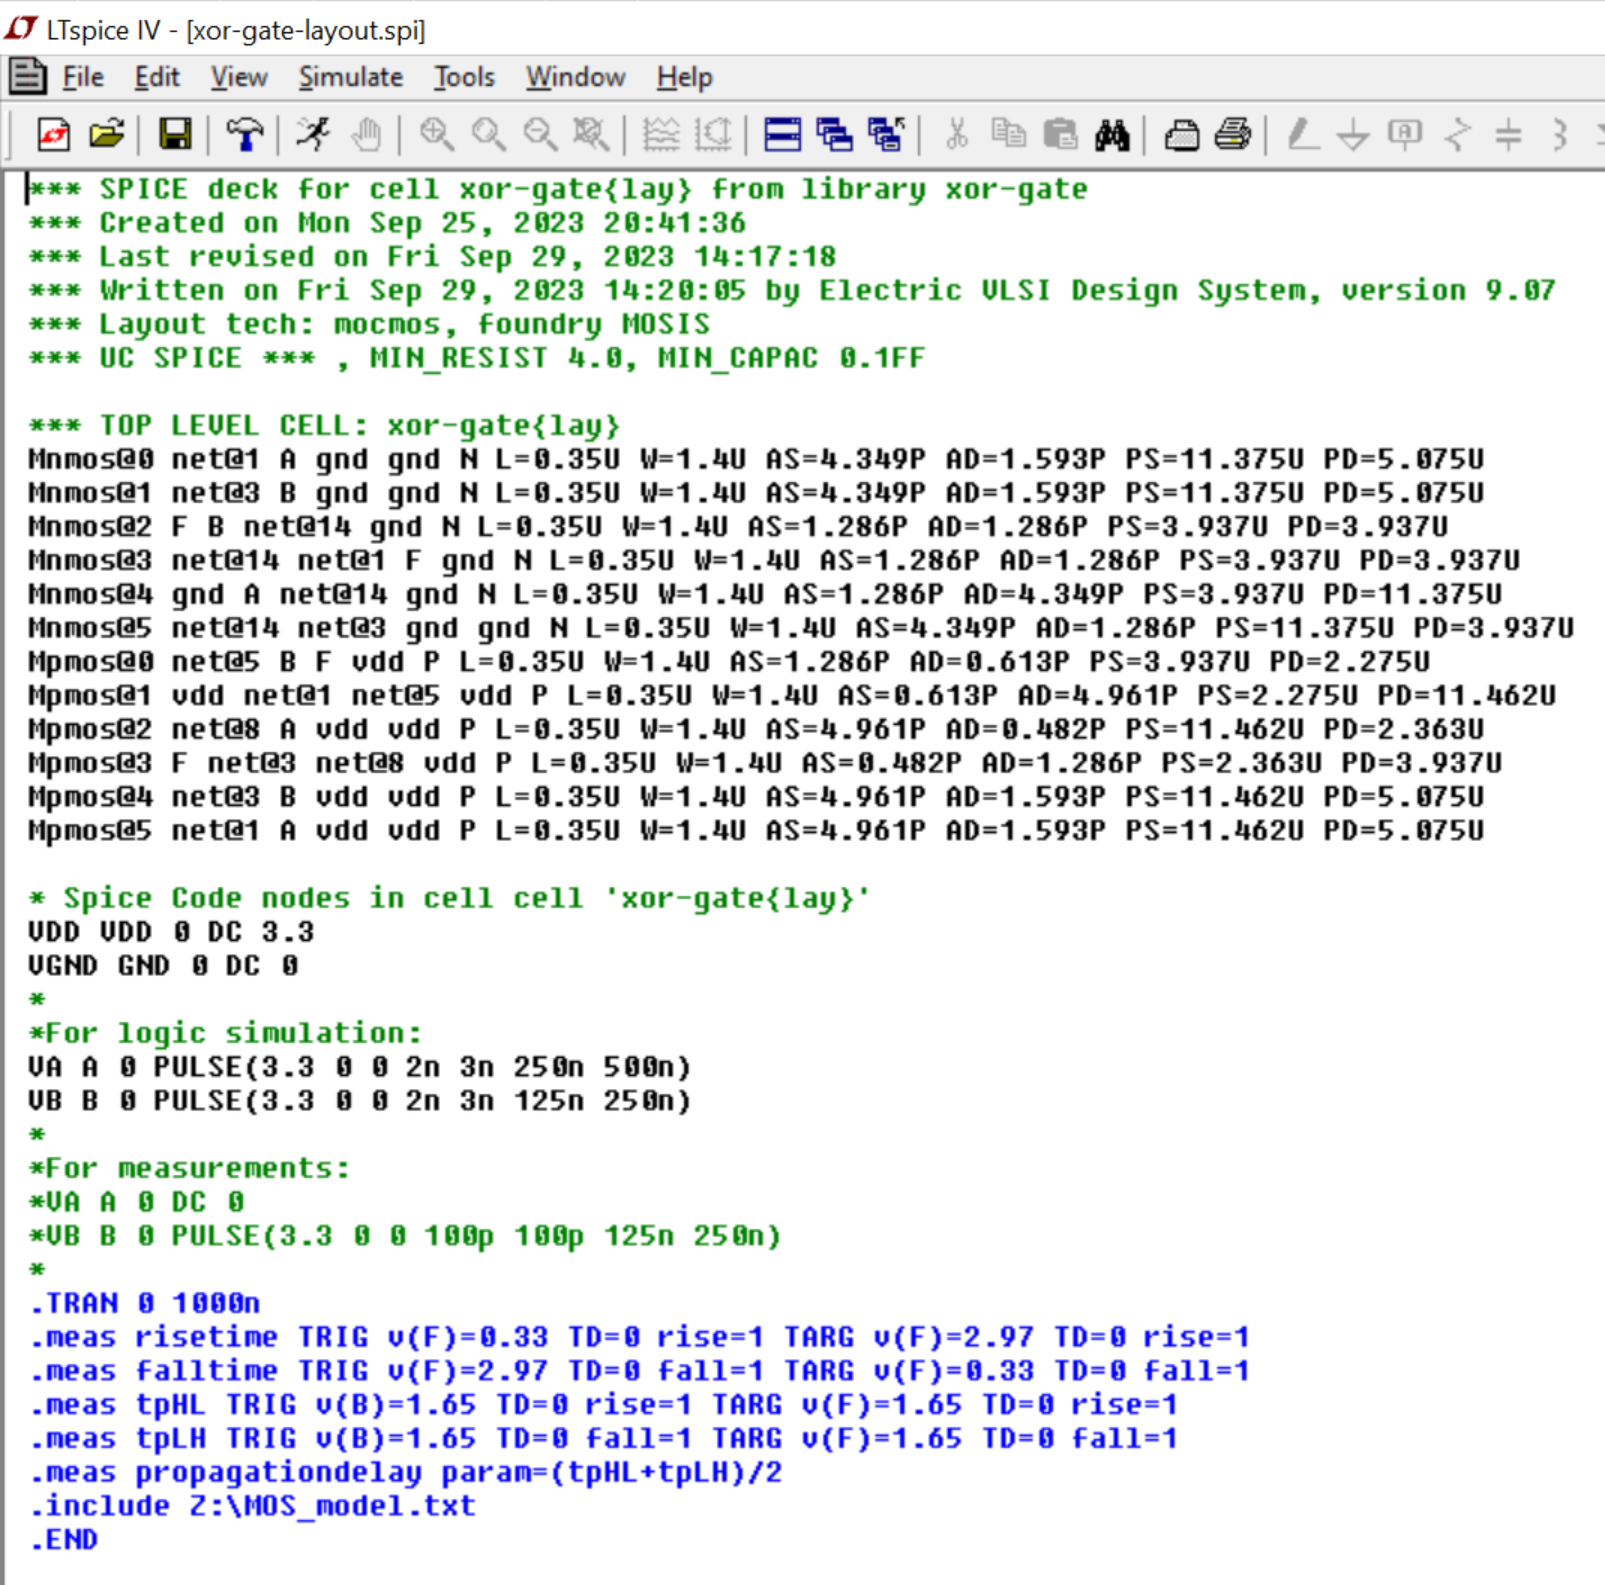
\includegraphics[width=0.9\linewidth, frame]{screenshots/spice-layout.png}
    \caption{The spice code for simulating the layout of the XOR gate.}
    \label{fig:spice-lay}
  \end{figure}

  \paragraph{}
  The resulting waveforms from the spice simulation of the XOR gate layout are shown in Figure \ref{fig:spice-sim-lay}. This shows the same correct behavior we saw in Table \ref{table:xor} and the simulation of the schematic in Figure \ref{sch-sim}.


  \begin{figure}[H]
    \centering
    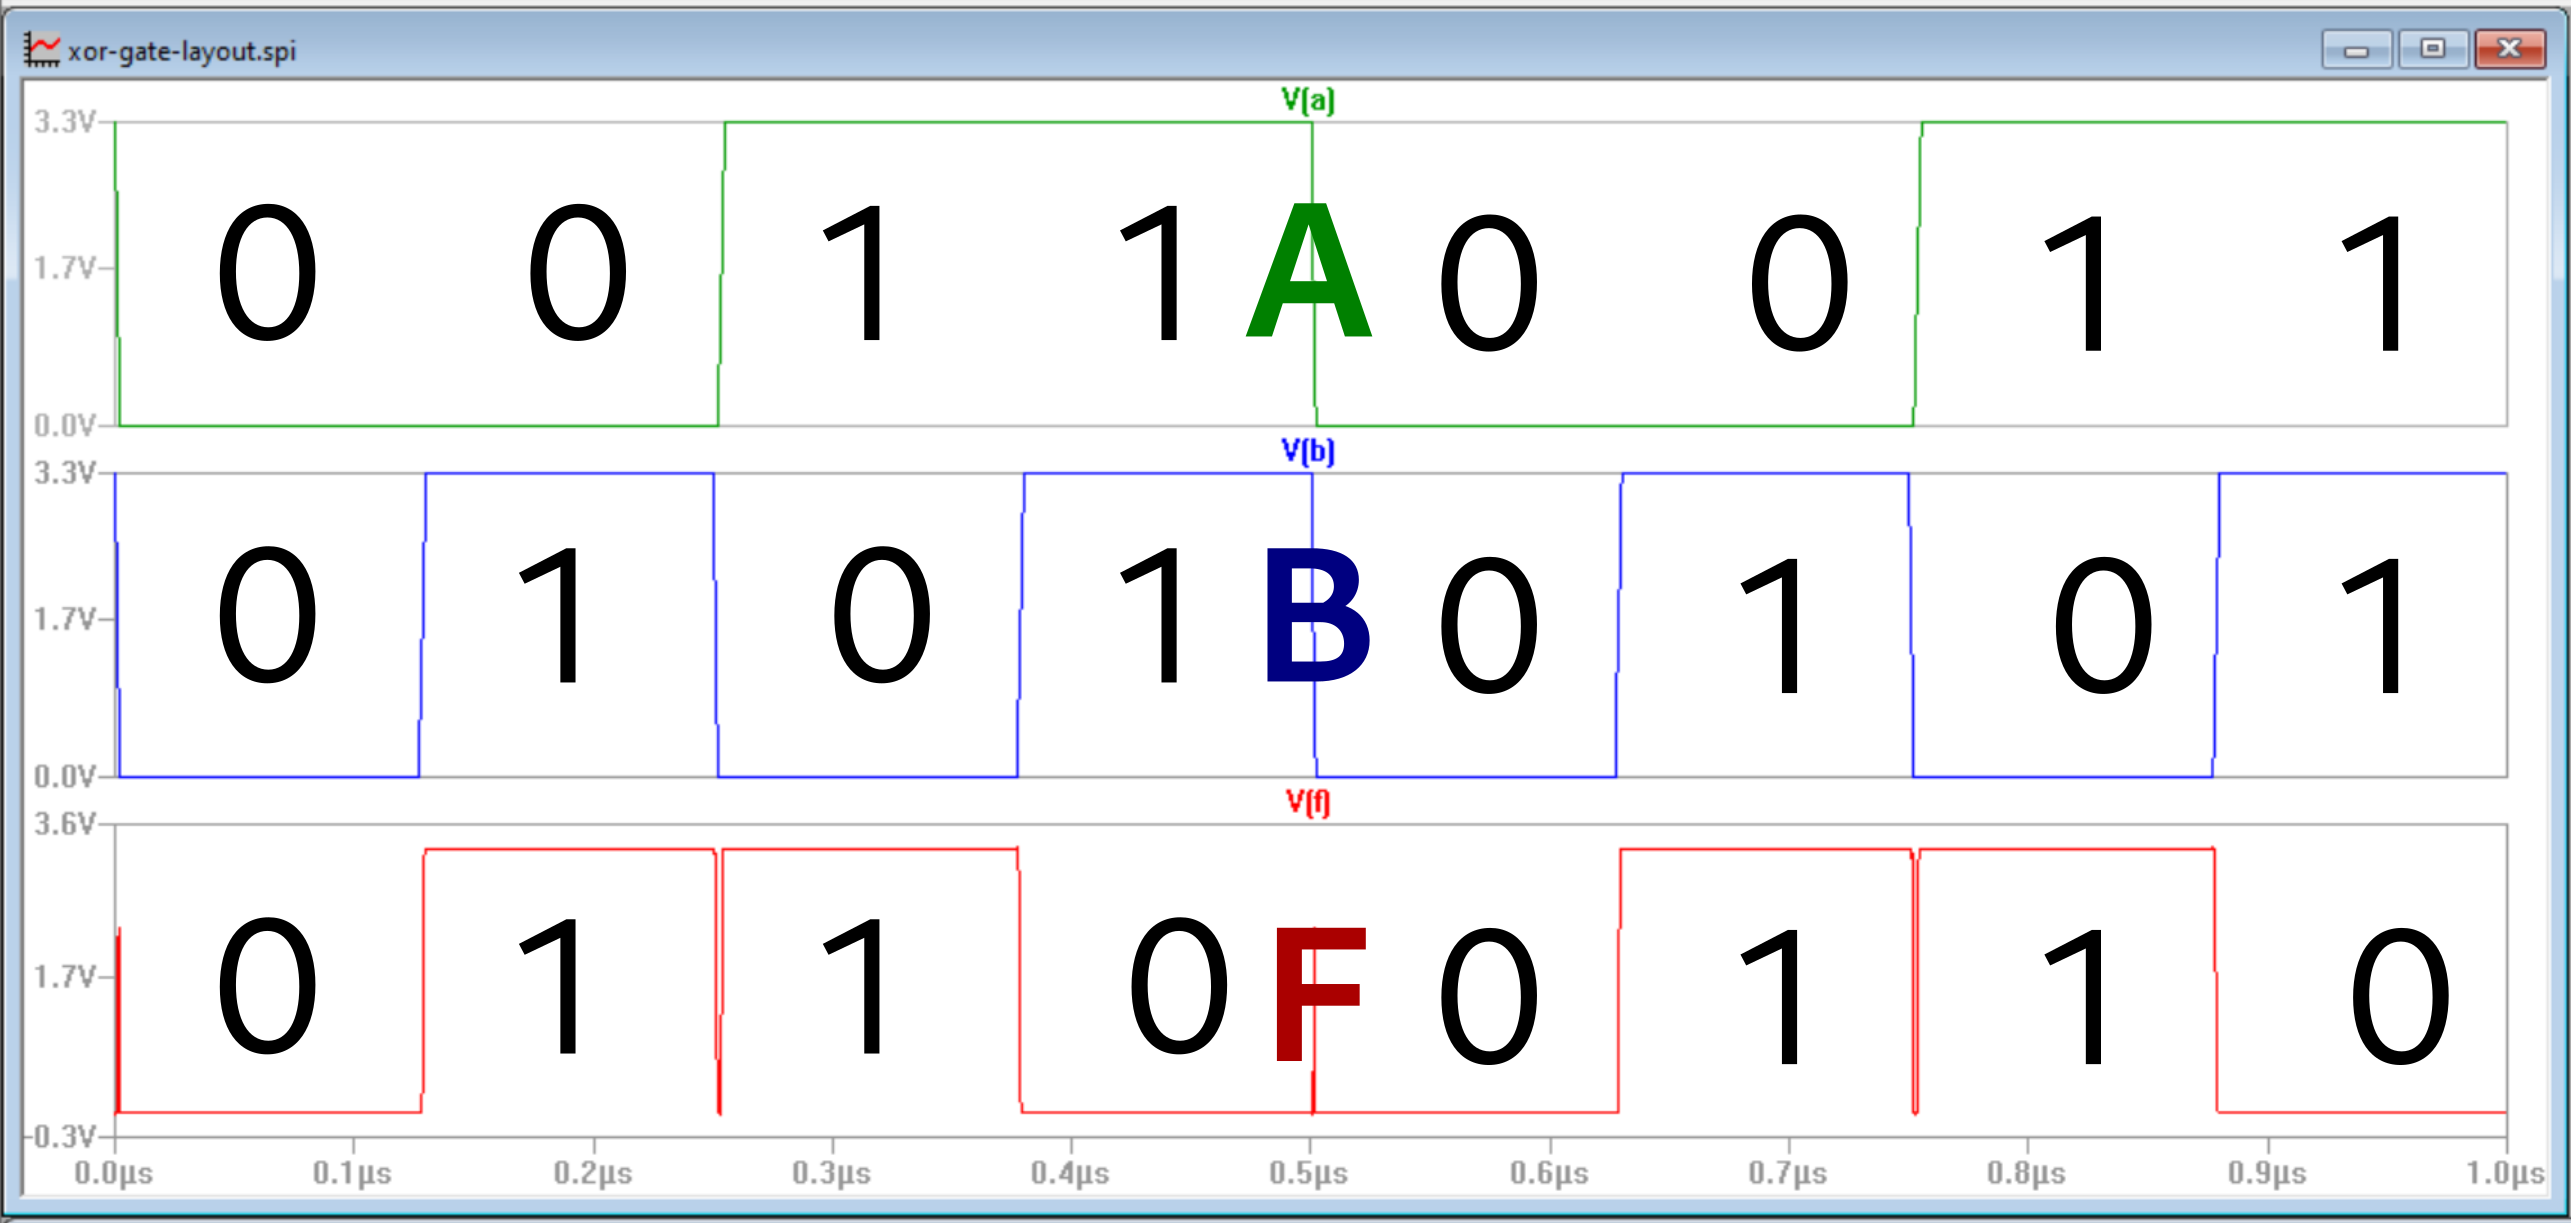
\includegraphics[width=0.9\linewidth, frame]{screenshots/spice-sim-layout.png}
    \caption{The resulting graphs from the spice simulation of the XOR gate layout.}
    \label{fig:spice-sim-lay}
  \end{figure}

  \paragraph{}
  The IRSIM simulation also follows the same procedure as with the schematic. The results for the IRSIM simulation are shown in Figure \ref{fig:irsim-lay}. The results are correct and match the simulation from LTSpice in Figure \ref{fig:spice-sim-lay} and the logic shown in Table \ref{table:xor}.



  \begin{figure}[H]
    \centering
    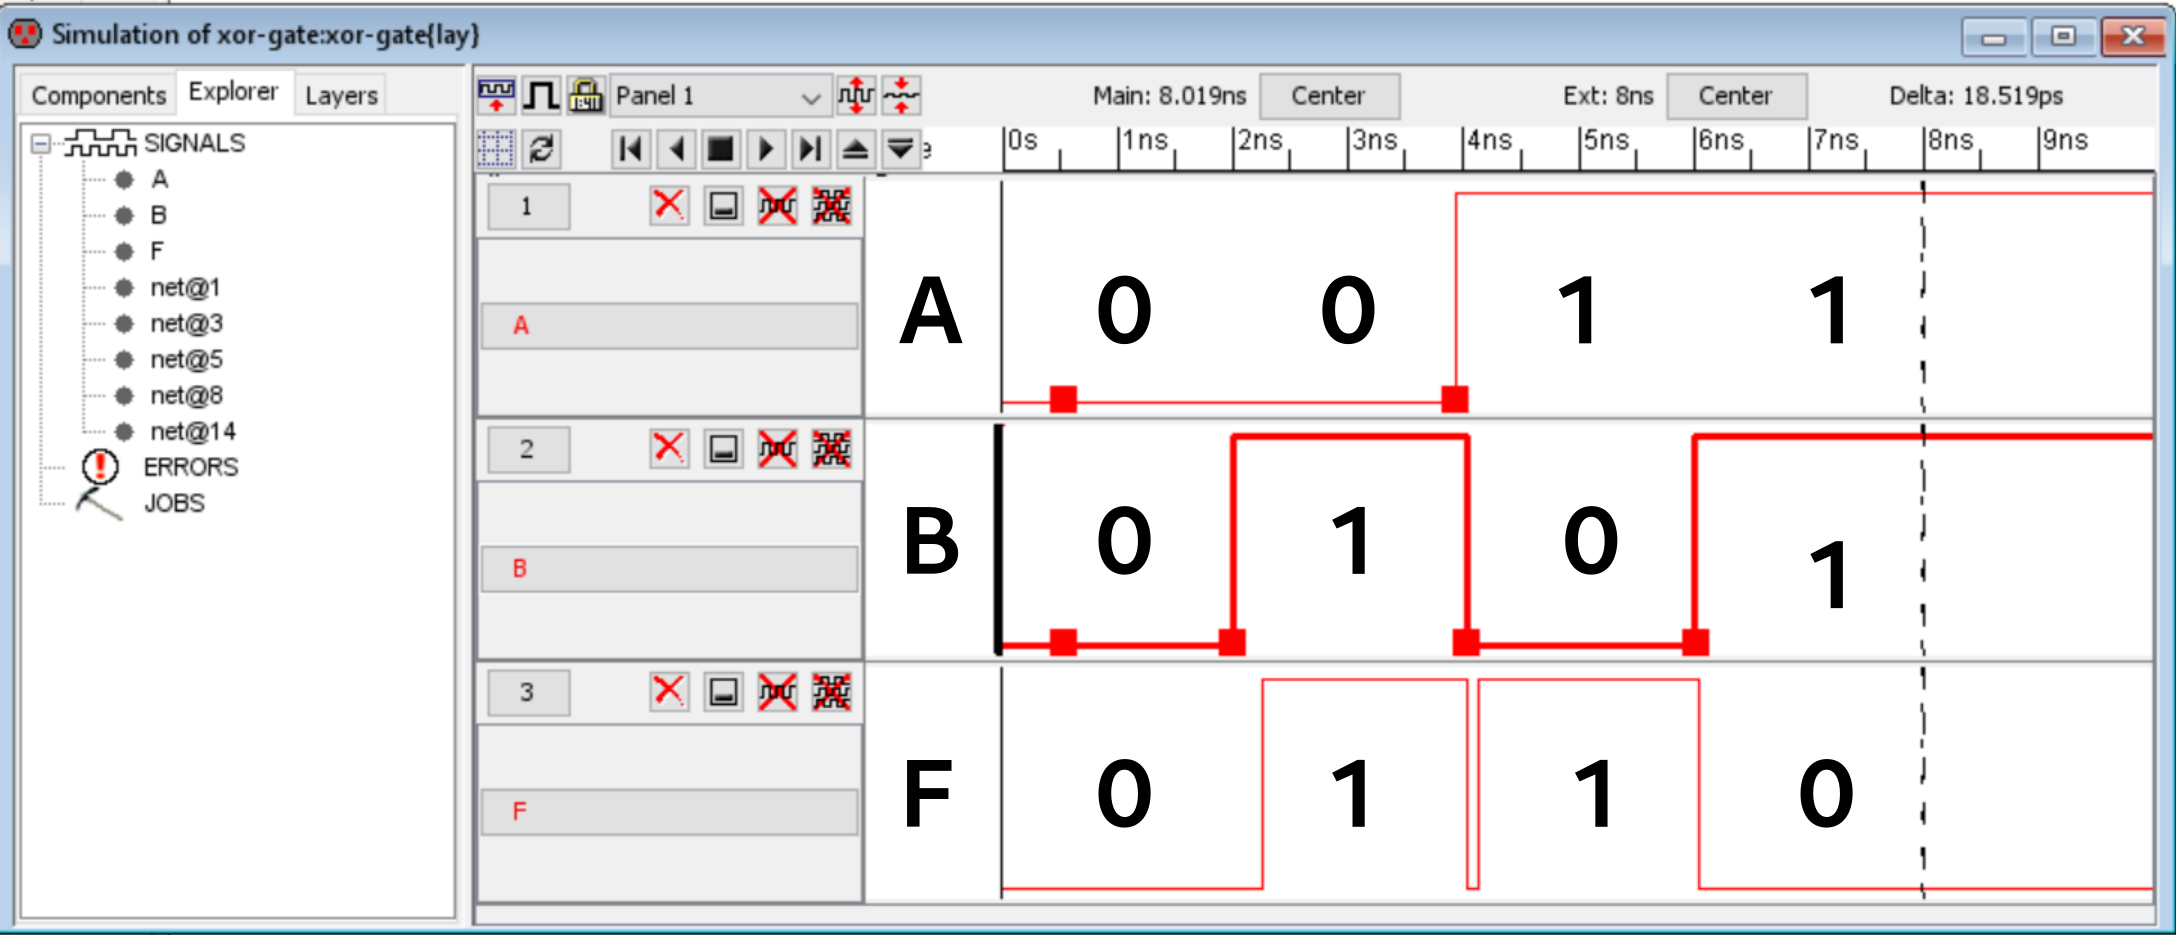
\includegraphics[width=0.9\linewidth, frame]{screenshots/irsim-layout.png}
    \caption{The resulting graphs from the IRSIM simulation of the XOR gate layout.}
    \label{fig:irsim-lay}
  \end{figure}

\section{Layout Measurements}
  \paragraph{}
  The same measurements are taken using LTSpice with the same procedure as detailed for the schematic. The spice code for taking these measurements is shown in Figure \ref{fig:spice-meas-lay}.


  \begin{figure}[H]
    \centering
    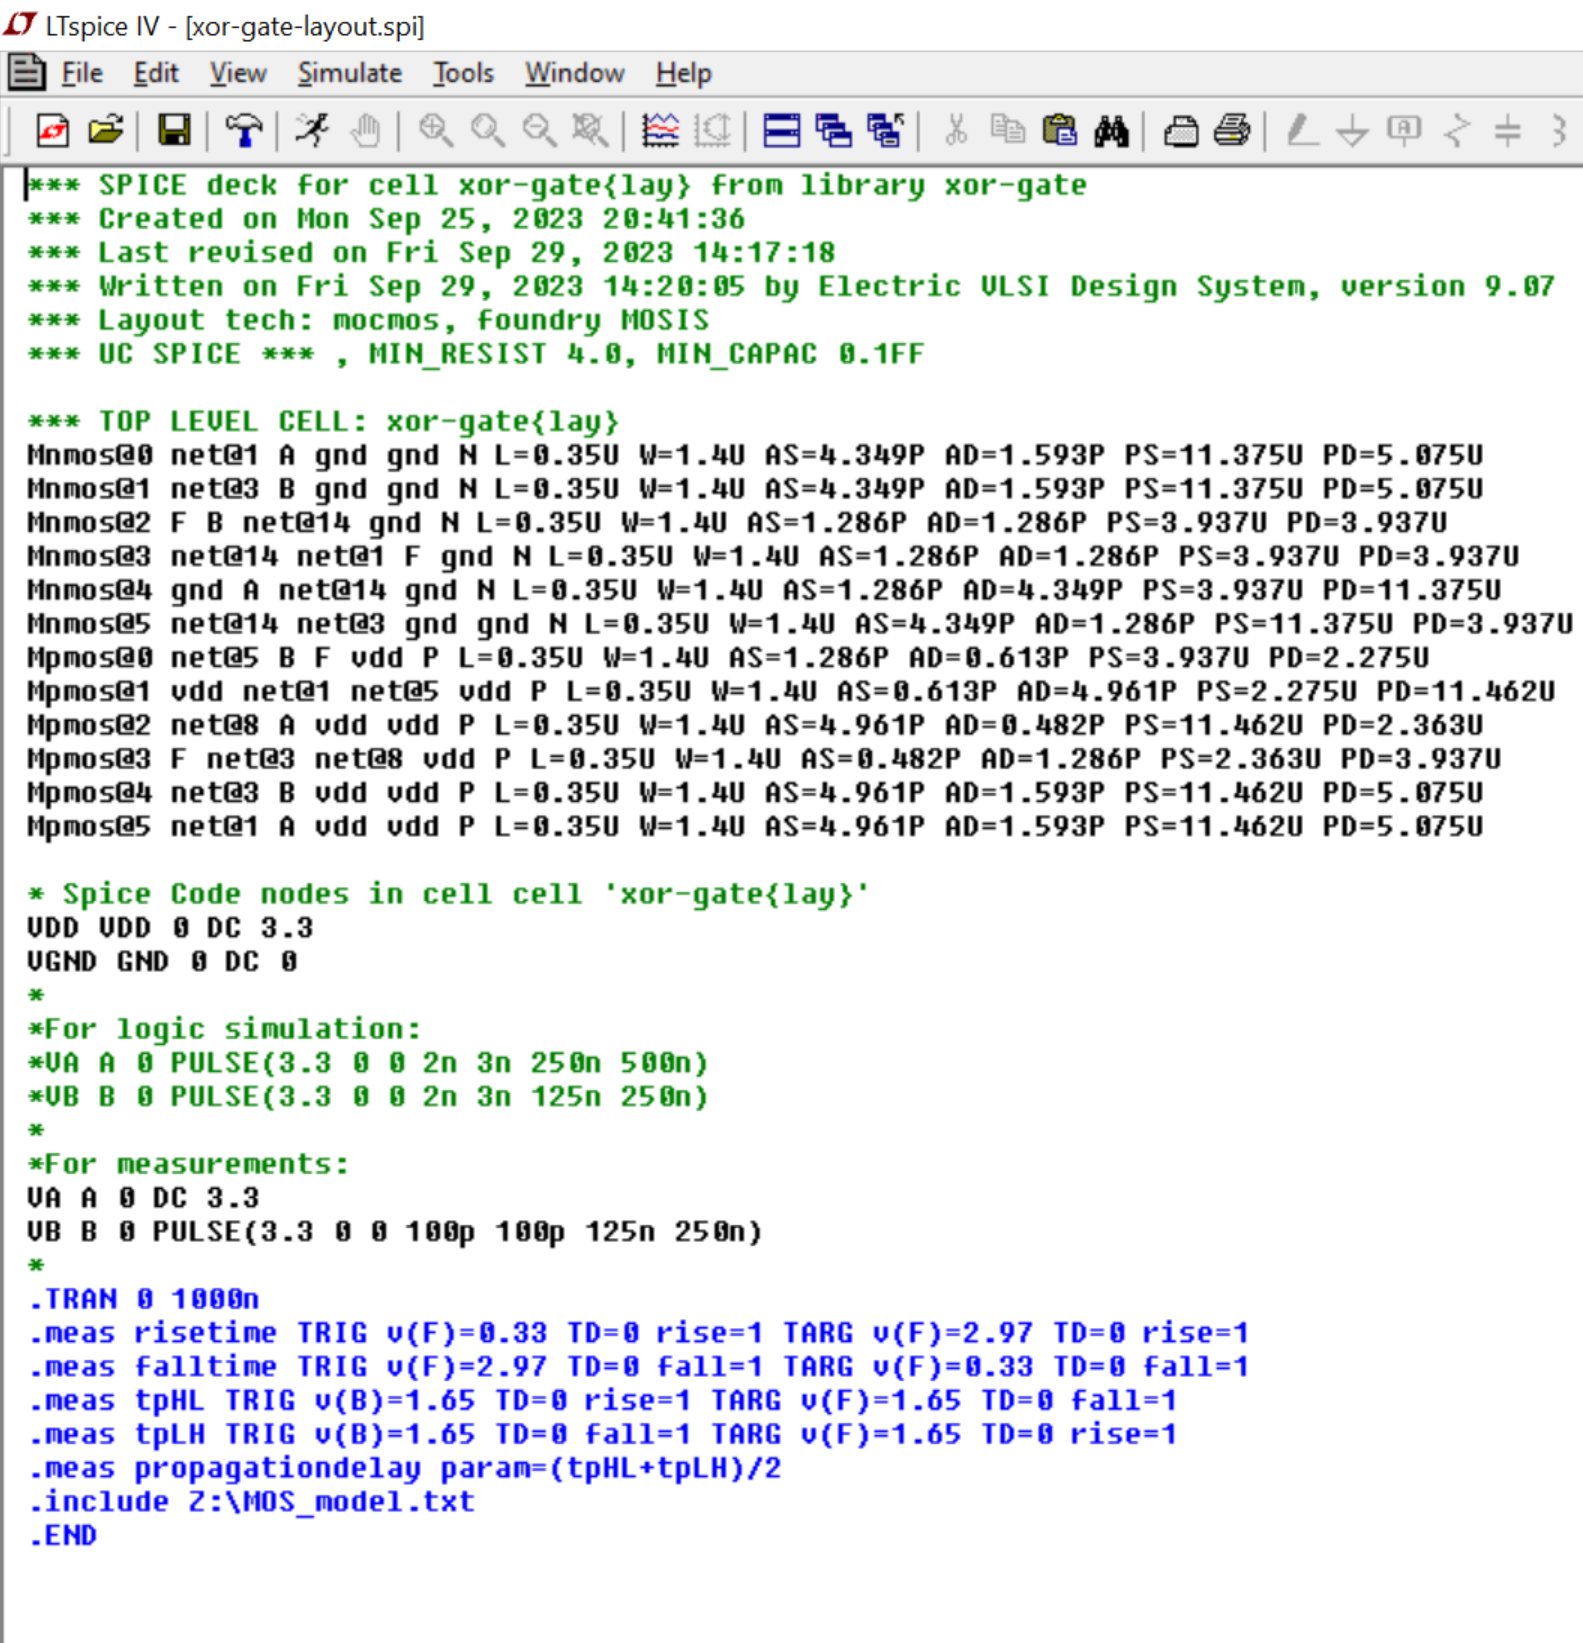
\includegraphics[width=0.9\linewidth, frame]{screenshots/spice-meas-layout.png}
    \caption{The spice code that measures the rise time, fall time, and propagation delay of the output signal of the XOR gate layout.}
    \label{fig:spice-meas-lay}
  \end{figure}





\begin{comment}
%How to do inline code:
\paragraph{}
There is some inline code, \inlinecode{movff STATUS, STATUS\_TEMP}, in this sentence.

This formula $f(x) = x^2$ is an example of inline math.

\end{comment}


\begin{comment}
%How to do equations:

\begin{equation*}
P_{1f_m}=\int^\infty_{-\infty}G_{1f_m}(f)df=0.01\int^\infty_{-\infty}[\delta(f-2700)+\delta(f-2300)]df=0.01*(1+1)=0.02W
\end{equation*}


\end{comment}


\begin{comment}

%Here is a single figure
\begin{figure}[H]
  \centering
  \includegraphics[width=0.9\linewidth, frame]{screenshots/01.png}
  \caption{The system for this lab.}
  \label{fig:01}
\end{figure}

\end{comment}

\begin{comment}

%Here is a double figure
\begin{figure}[H]
  \centering
  \begin{subfigure}[b]{0.45\linewidth}
    \includegraphics[width=\linewidth, frame]{screenshots/02.png}
    \caption{The xyz block.}
  \end{subfigure}
  \begin{subfigure}[b]{0.45\linewidth}
    \includegraphics[width=\linewidth, frame]{screenshots/03.png}
    \caption{The abc block.}
  \end{subfigure}
  \caption{The two figures in this double figure.}
  \label{fig:02}
\end{figure}

\end{comment}


\end{document}
